\documentclass[sigconf]{acmart}
\usepackage[flushleft]{threeparttable}
\usepackage[shortlabels]{enumitem}
\usepackage{subfigure}

\AtBeginDocument{%
  \providecommand\BibTeX{{%
    \normalfont B\kern-0.5em{\scshape i\kern-1000.25em b}\kern-0.8em\TeX}}}

\setcopyright{acmcopyright}
\copyrightyear{2022}
\acmYear{2022}
\acmDOI{10.1145/1122445.1122456}

\acmConference{May 5-5-22, 2022}{Moscow, Idaho, USA}
%\acmBooktitle{CIKM '22: 31st ACM International Conference on Information and Knowledge Management}
%\acmPrice{15.00}
%\acmISBN{978-1-4503-XXXX-X/18/06}

\begin{document}

\title{Best Buy Search Final Report}

\author{Seth Cram}
\affiliation{%
  \institution{University of Idaho}
  \streetaddress{875 Perimeter Drive}
  \city{Moscow}
  \state{Idaho}
  \country{USA}
  \postcode{83843}
}
\email{cram1479@vandals.uidaho.edu}

\author{Chadwick Goodall}
\affiliation{%
  \institution{University of Idaho}
  \streetaddress{875 Perimeter Drive}
  \city{Moscow}
  \state{Idaho}
  \country{USA}
  \postcode{83843}
}
\email{good0206@vandals.uidaho.edu}

\begin{abstract}

This document focuses on the creation and development of a Best Buy service matching database project assigned in CS 360 at the University of Idaho. The overarching goal of the project was to implement a web-service that would match products and services offered by vendors to a customer, through the creation of a website. This was accomplished using the Django web framework, the MySQL relational database management system and several other web development tools and frameworks. 

Brief Disclaimers: The words "product" and "item" are used nearly interchangeably below. Since there's a category labeled as "services", all products should be assumed as "items". This has been an ongoing struggle to settle on the proper wording. Additionally, the words "model" and "table" are used interchangeably and should be treated as referring to the same structure.

\end{abstract}


\begin{CCSXML}
<ccs2012>
   <concept>
       <concept_id>10002951.10002952.10002953.10002955</concept_id>
       <concept_desc>Information systems~Relational database model</concept_desc>
       <concept_significance>500</concept_significance>
       </concept>
   <concept>
       <concept_id>10002951.10002952.10002953.10002959</concept_id>
       <concept_desc>Information systems~Entity relationship models</concept_desc>
       <concept_significance>300</concept_significance>
       </concept>
   <concept>
       <concept_id>10002951.10002952.10003197.10010822.10010823</concept_id>
       <concept_desc>Information systems~Structured Query Language</concept_desc>
       <concept_significance>500</concept_significance>
       </concept>
   <concept>
       <concept_id>10002951.10002952.10003212.10003216</concept_id>
       <concept_desc>Information systems~Autonomous database administration</concept_desc>
       <concept_significance>300</concept_significance>
       </concept>
   <concept>
       <concept_id>10002951.10002952.10003190.10003205</concept_id>
       <concept_desc>Information systems~Database views</concept_desc>
       <concept_significance>500</concept_significance>
       </concept>
   <concept>
       <concept_id>10002951.10002952.10003400.10003401</concept_id>
       <concept_desc>Information systems~Database web servers</concept_desc>
       <concept_significance>500</concept_significance>
       </concept>
 </ccs2012>
\end{CCSXML}

\ccsdesc[500]{Information systems~Relational database model}
\ccsdesc[300]{Information systems~Entity relationship models}
\ccsdesc[500]{Information systems~Structured Query Language}
\ccsdesc[300]{Information systems~Autonomous database administration}
\ccsdesc[500]{Information systems~Database views}
\ccsdesc[500]{Information systems~Database web servers}


\keywords{RDMS (Relational Database Management System), ER (Entity Relation) diagram, MySQL, Django, Bootstrap, PHPMyAdmin, Python, HTML, JS, CSS, items, products}

\maketitle


\section{Introduction}

\paragraph{In today's modern world almost all software is a service and most companies implement some form of web-service to conduct business. The students of CS360 were given the task of creating a database solution for a product/service matching third party service provided for Best Buy. The stipulations of the project description included that a customer must be able to anonymously (relative to vendors) disclose their product/service requirements under terms and conditions of service and then customers should be able to receive a "wish-list" of their items. This wish-list, which for our particular application was implemented in the form of search pages, was required to display a perfect match to the customer's search and a closest similar match. A requirement match was achieved through a different type of page, a recommendations page based on customer cart items. With this in mind, similar to many businesses, the approach taken was to implement a web-service application. Therefore, the Best Buy Search website was developed.}

\paragraph{This service implements account registration under a binding contract of terms and conditions of service, as well as several searching and filtering capabilities that are provided to the user of the website, either customer or vendor, as well as a cart for customers to add and remove items from for checkout. Additionally, vendors are able to fully utilize the CRUD operations in order to Create, Read, Update, or Delete listed products on the site.}

\subsection{Design}

\begin{figure}[H]
    \centering
    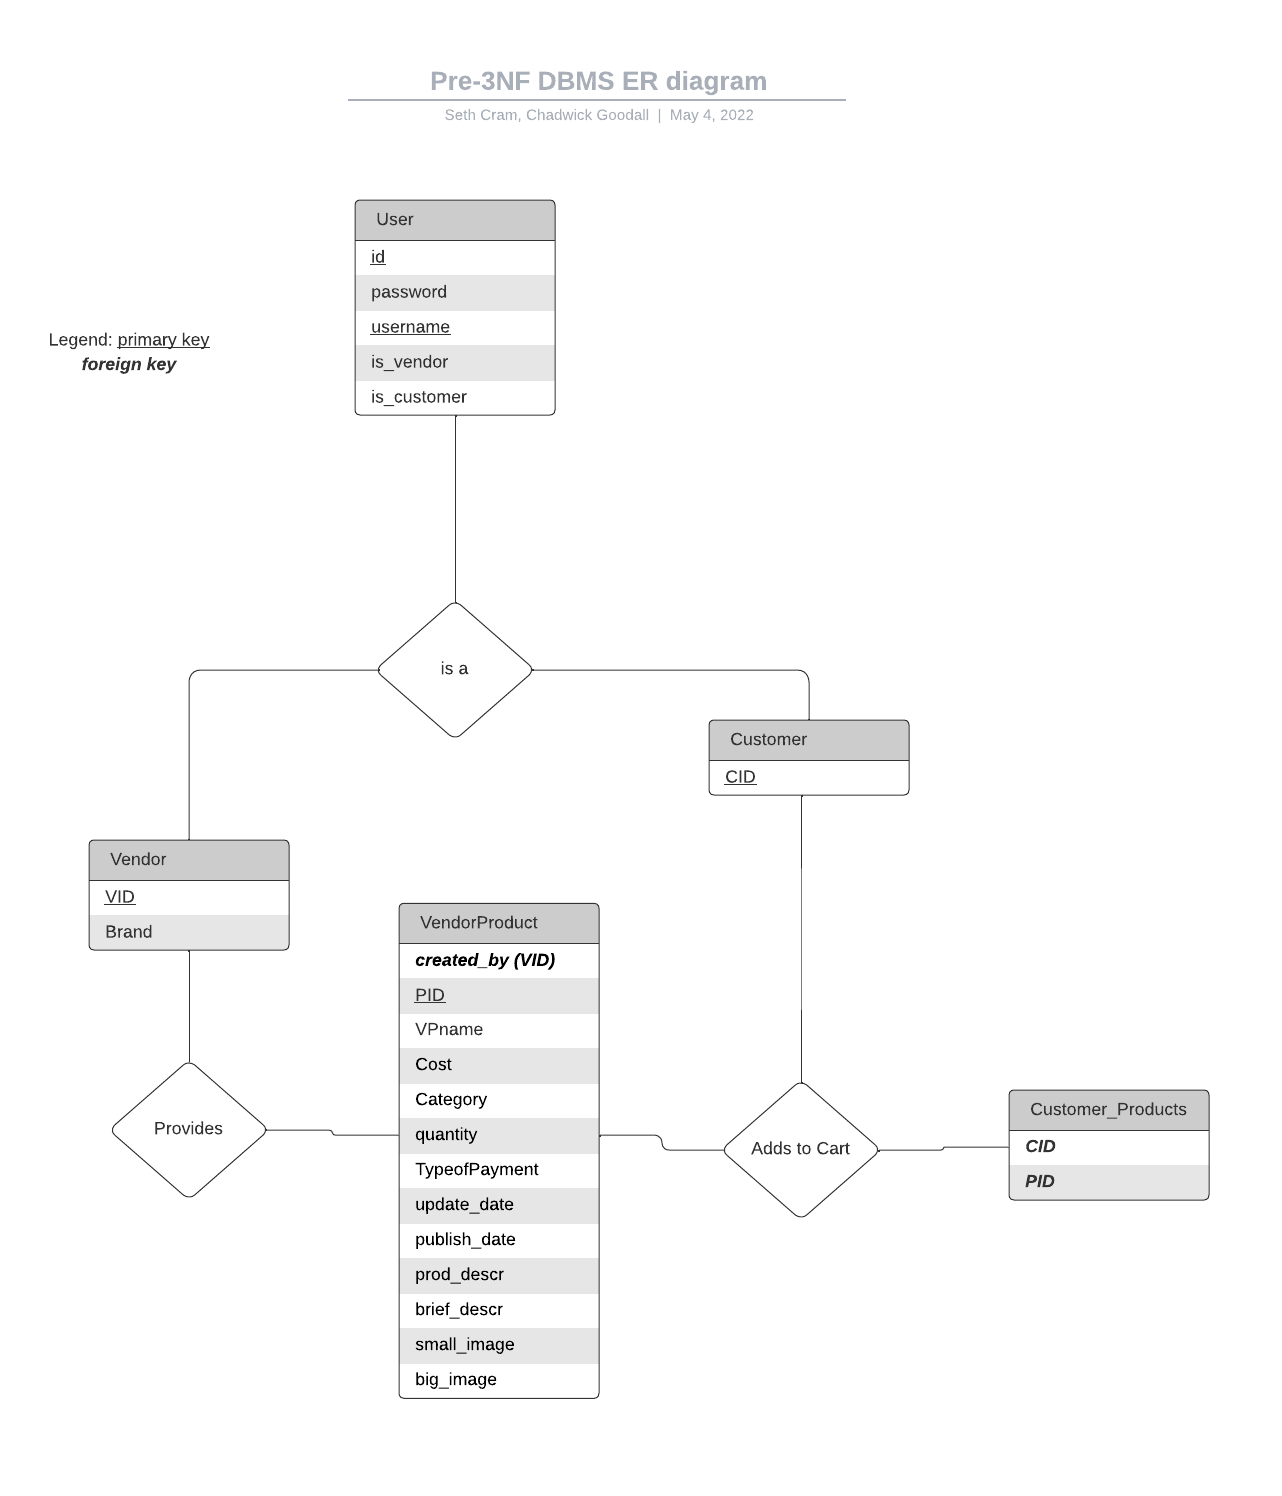
\includegraphics[scale=0.4]{Pre_Post-3NF DBMS ER diagram (UML notation) (2).png}
    \caption{Pre 3NF Decomposition Diagram}
    \label{fig:my_label}
\end{figure}


\paragraph{ The design of the Best Buy Search database consists of five tables: User, Vendor, Customer, CustomerProduct and VendorProduct. The first three tables serve as determining what permissions a site visitor should have. The CustomerProduct table links customers to what items they've decided to add to their cart. Finally, the VendorProduct table contains all information related to published items and necessary for display. }

\paragraph{ As seen above, the design modeling of Best Buy Search adheres to the pre-3NF decomposition, rather than the post-3NF decomposition schema. Throughout the rest of the report, several reasons are given for this discrepancy. The main reason being that for future expand-ability, keeping the Customer table is crucial. To dissuade possible doubt, the separation of the Customer id into its own table shouldn't enable update, insertion, or deletion anomalies, since the post-3NF decomposition schema can be ordered in several ways, one being equivalent to the ER Diagram used in the Best Buy Search database. }

\begin{figure}[H]
    \centering
    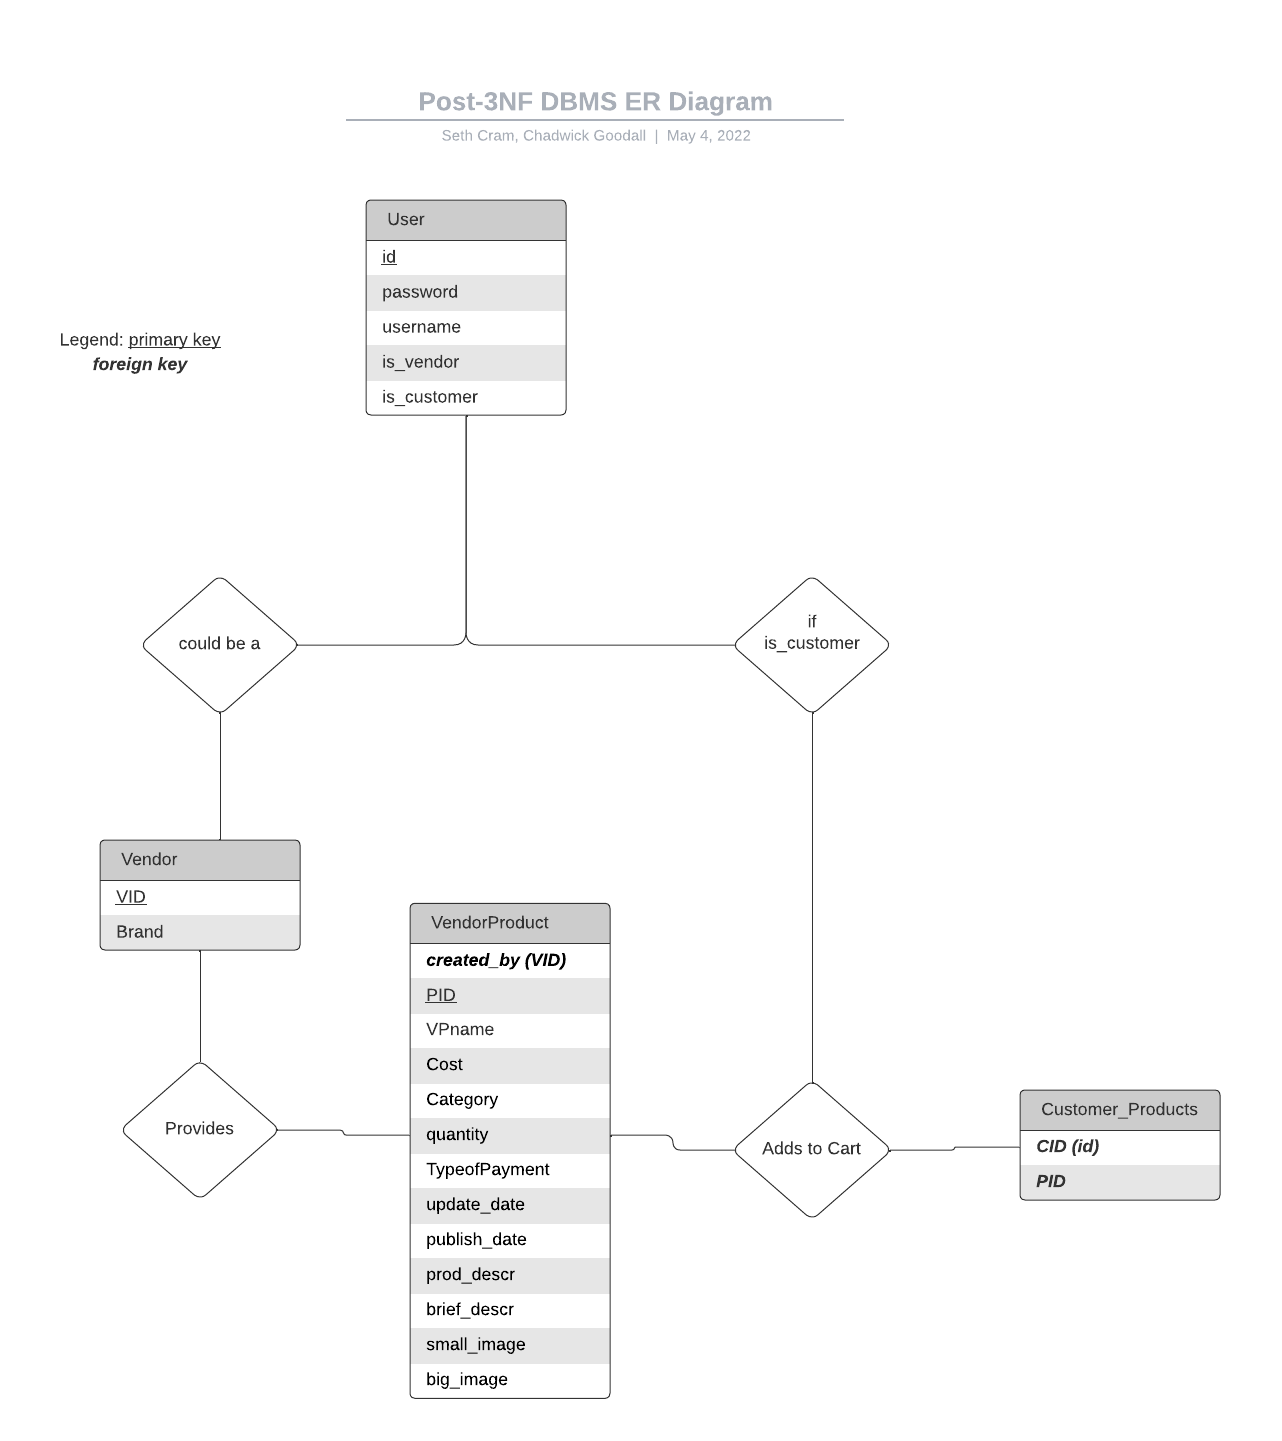
\includegraphics[scale=0.4]{Pre_Post-3NF DBMS ER diagram (UML notation) (4).png}
    \caption{Post 3NF Decomposition Diagram}
    \label{fig:my_label}
\end{figure}

\paragraph{ Database design began at a strictly abstract level and the ER diagram initially contained around eight tables. Upon realizing that a variety of tables needed to fulfill the search requirements were derive-able and not contained within the database, the diagram shrunk in size. }

% do not know what to put here yet

\subsection{Tools used for development}

\paragraph{Throughout the development of this project, several software tools were necessary for the completion of the Best Buy Search web-service. Some of these tools that were used include the XAMPP web server solution for locally hosting the MySQL database and providing the PHPMyAdmin service. PHPMyAdmin was an integral tool, providing visibility into the database and its tables over the course of development and was used to view resulting table changes and test the functionality of pages within the website. This was primarily necessary to ensure that the website was properly interacting with the database and vice versa. The actual coding environments used for programming the project primarily relied upon Spyder, Visual Studio, and Visual Studio Code. Git, as well as the accompanying webservice Github, were used for version control of the project to ensure project files were in sync between both developers at all times.}

\paragraph{The backend framework, which is the driving force behind most of the project, was the Django web framework which is implemented using Python3. Django allows for the implementation of a model-template-view architectural pattern and, with a basic knowledge of Python classes, allows for the rapid development of web based applications. The template aspect of Django's development architecture allowed for the inheritance of structure and style when developing the UI. This greatly assisted in speeding up the development of the website. Furthermore, Django was also chosen for the development of this project since it was written in Python, which both team members have experience coding in.}

\paragraph{The frontend framework used to design and implement the user interface was the free and open source Bootstrap CSS framework. With ample documentation and boilerplate code, Bootstrap facilitated the development of the UI (User Interface) and expedited the creation of the webpages themselves tremendously. Utilizing bootstrap's available resources enabled both developers, with minimal knowledge of most web development languages such as HTML, CSS, and JavaScript, to create a sleek, modern, and feature-rich interface for the Best Buy Search service.}
  

\subsection{Languages used for development}

\paragraph{The languages used to develop the Best Buy Search were primarily dictated by the tools (frameworks) that were used to develop it. As such, Python was the main language used for programming the facilitated functionality of the website built on Django. Python, being a rather human readable and vastly practical and applicable programming language, was chosen due to its ease of use as well as both programmers having extensive experience with the language. HTML, CSS, and Javascript were primarily imported from the Bootstrap frontend framework and enabled the website's ease-of-use and stylization which included buttons, the navigation bar, search bar, forms, drop-down menus, etc. As stated previously, with both developers having rather minimal experience in web development, the framework facilitated design and vastly abstracted the nuances behind a majority of the process.}

\section{Best Buy Search Database}

\paragraph{As with most databases, the Best Buy Search database schema is composed of several tables containing data relevant to the implementation and functionality of the project. With the given criteria that the project is supposed to implement a product/service matching service for Best Buy, tables were constructed to properly implement such a project that involved keeping track of the users and items. To manage all of the necessary data, product vendors, and customers, the following tables were constructed in order to manage their related information: user, customer, customer products (implements the customer's shopping cart), vendor, and vendor products. The following text describes and discusses the implementation, contents, and importance of each of these tables in the overall design of the Best Buy Search service.}

\subsection{User table}

\paragraph{The user table contains information shared by both customer and vendor user types. It contains the user ID, password, username, is\_vendor, and is\_customer. Both is\_vendor and is\_customer are boolean fields used to determine a whether a user is a vendor or customer. ID and username serve as two primary keys in the user table, which may seem redundant. An argument for keeping both primary keys is that username needs to be unique for verification purposes and cannot contain null values, and ID was kept as a primary key in the event of converting over to using email for login verification instead of username. Email itself wouldn't necessarily have to be a primary key, and it would make resetting passwords much easier to implement.}     

\paragraph{In retrospect, the is\_vendor and is\_customer fields seem fairly redundant, since the vendor and customer tables can also serve the purpose of differentiating whether a user is a customer or not. Thus it makes sense why these fields were removed from the left-hand-side of all the functional dependencies during the 3NF Decomposition. Therefore, a recommendation for further development would be to entirely remove the is\_vendor and is\_customer fields, and rewrite the decorators that use these fields to take advantage of all three user tables. }

\subsection{Customer table}

\paragraph{The customer table within the database schema manages and keeps track of the customer accounts that have been registered to the Best Buy Search site. As a result, this table is a rather simple list of customer IDs. }

\paragraph{When performing the 3NF decomposition, it was possible to combine this table into other pre-existing tables, but it was kept apart simply for future expansion when the customer has more fields unique to them. Credit card and address information are important fields for the creation of a fully-functioning checkout page and may be unique to the customer user type. }

\subsection{Customer products table}

\paragraph{The customer products table is used to implement a user's cart within the database schema. The vendor product IDs that the customer is checking out as well as the customer ID is stored within this table. By using this method to store this data, it allows a specific product or products to be associated with a particular customer. Since this data is then managed by the database, the customer is free to browse through all of the products and leave the website without losing the items in their cart. }

% not sure what just 'id' is
% it's unnecessary, but Django added it by default since the table wouldn't have a primary key otherwise

\subsection{Vendor table}

\paragraph{The vendor table includes the pieces of information required to identify a vendor which includes the user ID as well as the vendor brand. The brand name information is provided by the user upon vendor account creation within the system, however, it is not functionally implemented across the website. In future development, it would be possible to use the brand name for item display and as a search field.}

\subsection{Vendor product table}

\paragraph{The vendor product table keeps track of all of the products that are listed on the Best Buy Search site. This is easily the largest table managed by the database as each product registered to this table contains information such as the product ID number, name, cost, and type of payment for the product. Additional miscellaneous information is also stored for each product, which includes the date the item was published on the site, the date of its most recent update, the vendor ID that it was created by, and information for displaying itself on the shop page such as the quantity available, a brief and long product description, as well as display images. In further project expansion the "brand" field could also be stored in this table in order to allow the customer to  filter the products displayed in the shop by a specific brand.}

\paragraph{With the general concepts of the different tables necessary in order to implement the project, the next major portion to discuss is the user interaction with the service through the web interface.}

\section{Best Buy Search Interface}

\paragraph{An application user interface, when compared to the implementation of an application backend, is an equally important aspect to consider when developing a software service as it is the primary abstraction through which standard users will be able to accomplish varying tasks and go about their business.}

\subsection{Login page}

\paragraph{The login page is rather self explanatory and allows users, either customer or vendor, to login to their accounts. If the user does not yet have an account registered to the Best Buy Search database, they are provided the options to create an account as either a customer or item vendor to the site.}

\begin{figure}[H]
    \centering
    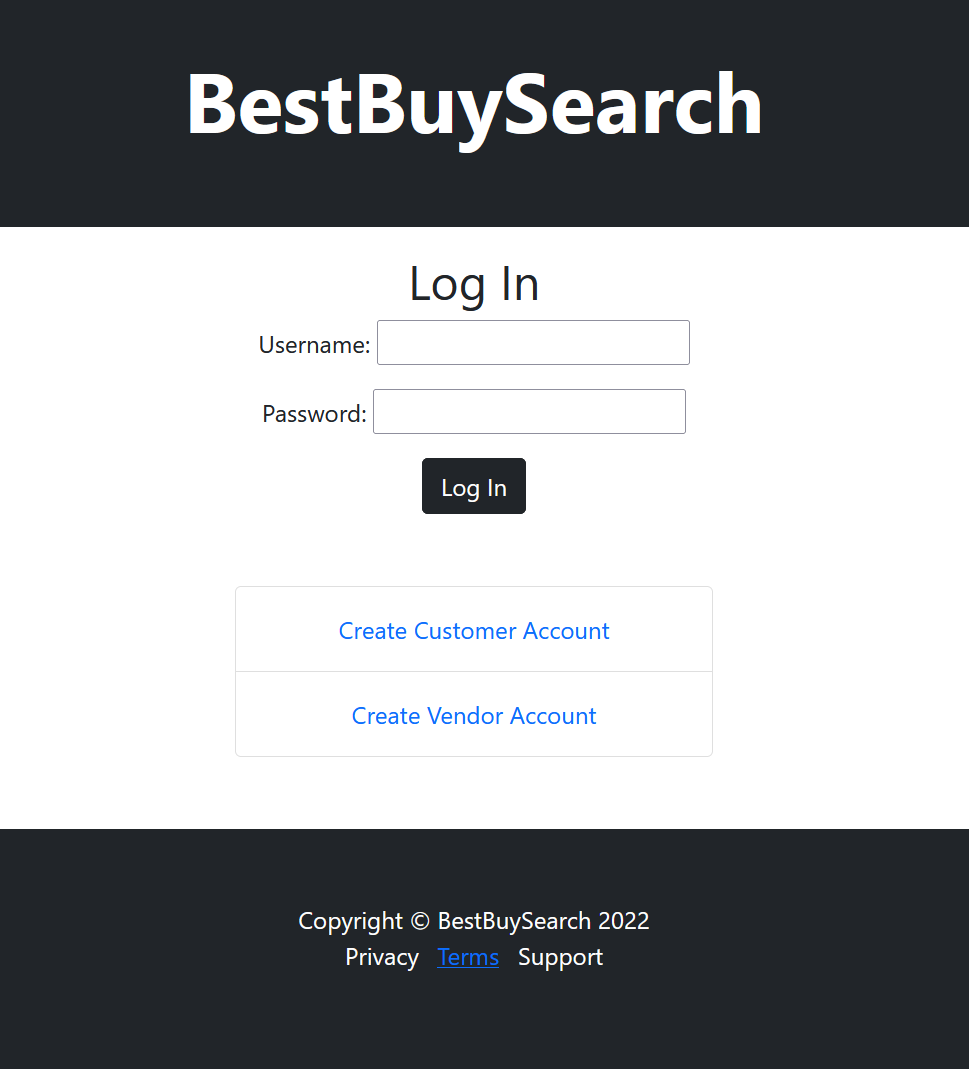
\includegraphics[scale=0.2]{login.PNG}
    \caption{User login homepage}
    \label{fig:my_label}
\end{figure}

\subsection{Customer account creation page}

\paragraph{The customer account creation page prompts the user for pertinent user information necessary for creating a Best Buy Search account, which includes a username and password. The page also states that the user's password must follow certain parameters for security purposes. Lastly, before creating an account, the user must agree to the terms and conditions of the Best Buy Search site.}

\paragraph{Inclusion of the user's requirement to agree to the terms and service of the site fulfills the project requirement of listing items under a "binding contract" that needs to be accepted by both the customer and vendor [1].}

\begin{figure}[H]
    \centering
    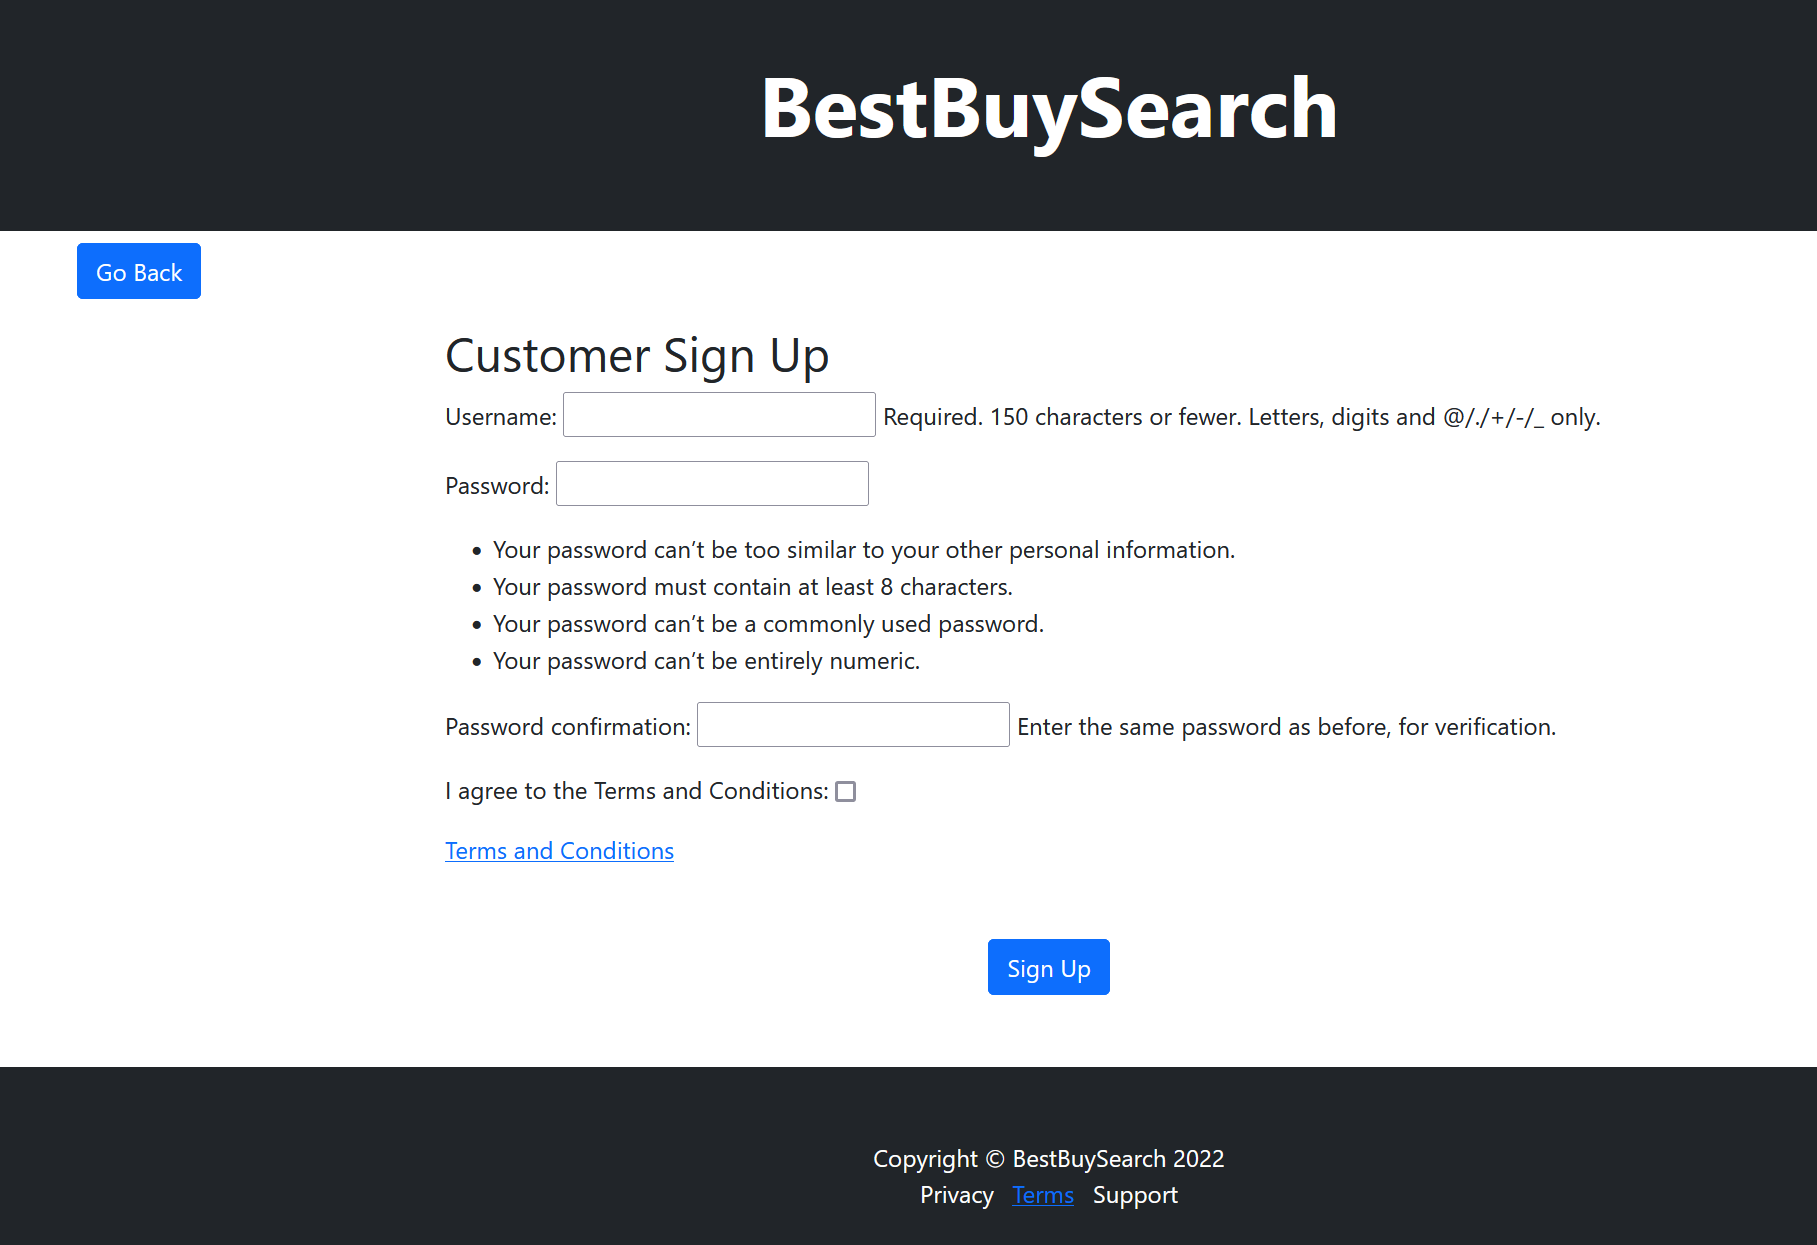
\includegraphics[scale=0.2]{CustomerSignup.PNG}
    \caption{Customer Sign up Page}
    \label{fig:my_label}
\end{figure}

\subsection{Vendor account creation page}

\paragraph{The vendor account creation page is similar to the customer account creation page, however, it requires additional information from the user in order to properly register an account. This additional information, on top of the username and password, is the brand name that will be associated with this vendor account. This is implemented in the Vendor table of the Best Buy Search database. As specified in the customer account creation page, the terms and conditions for the site must also be accepted by the vendor to create an account. }

\paragraph{Although not implemented, the brand name's original purpose was for displaying on each item. It would show the user who was selling the item, so they could make a more informed decision on what to purchase. Putting this concept into practice proved challenging, since the brand name is in the Vendor table and not the VendorProduct table. So, it never made it into the final product but should be considered for future development, which is why it was left in the website. }

\begin{figure}[H]
    \centering
    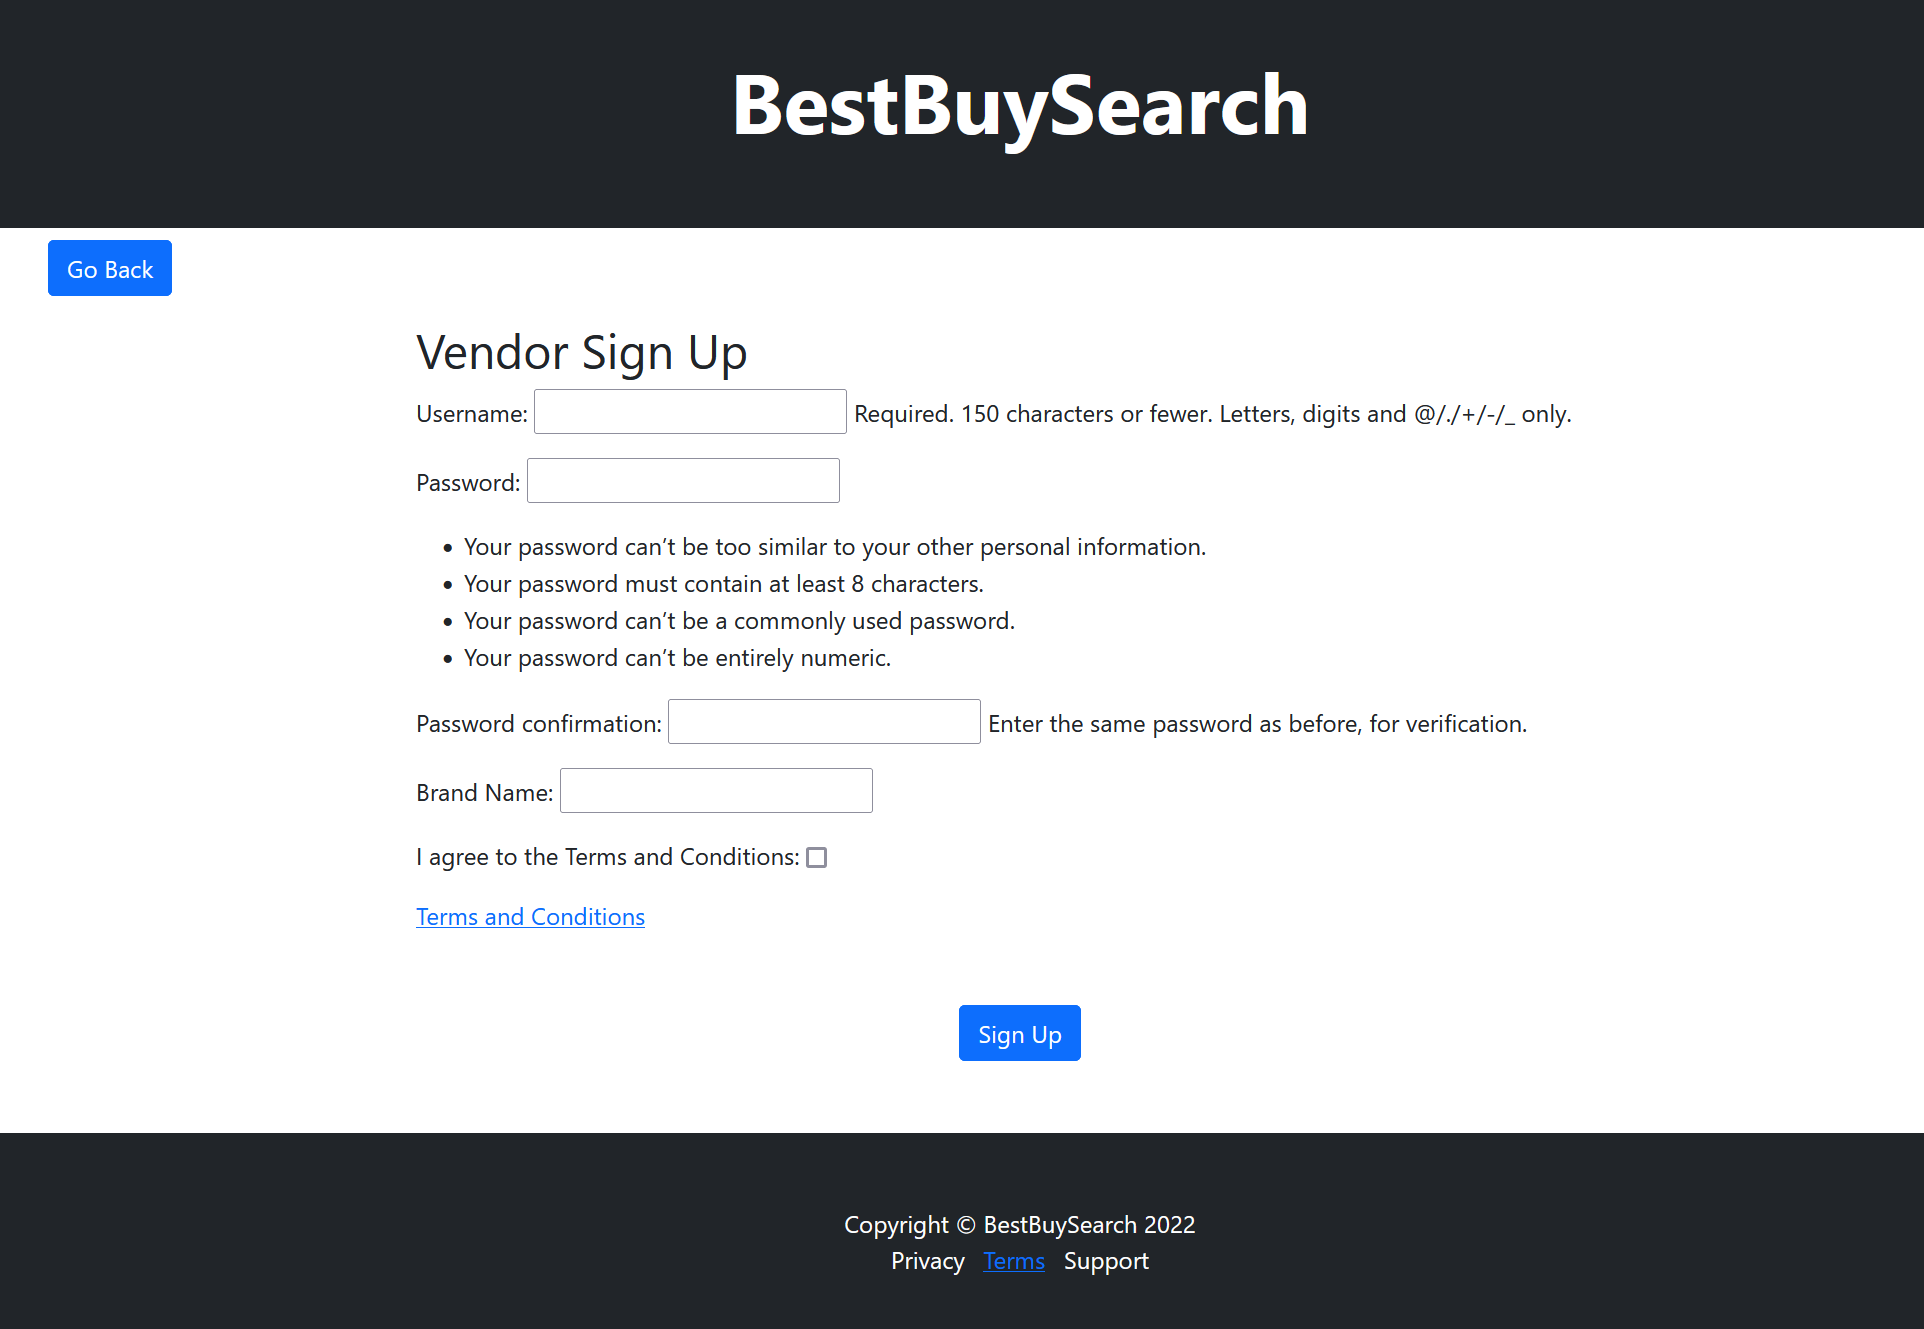
\includegraphics[scale=0.2]{VendorSignup.PNG}
    \caption{Vendor Sign up Page}
    \label{fig:my_label}
\end{figure}

\subsection{Home store page}

\paragraph{The home store page is kept intentionally bare to accommodate for quicker site navigation. It displays the four most recently updated vendor products and a link to the terms and conditions document users agreed to at the bottom of the page. The home page is the user's first introduction to the site after successfully creating and logging into an account, so their focus should be on the navigation bar. Depending on what type of user they've signed in as, they'll be able to navigate to a variety of different pages that'll be discussed in more detail below.}

\begin{figure}[H]
    \centering
    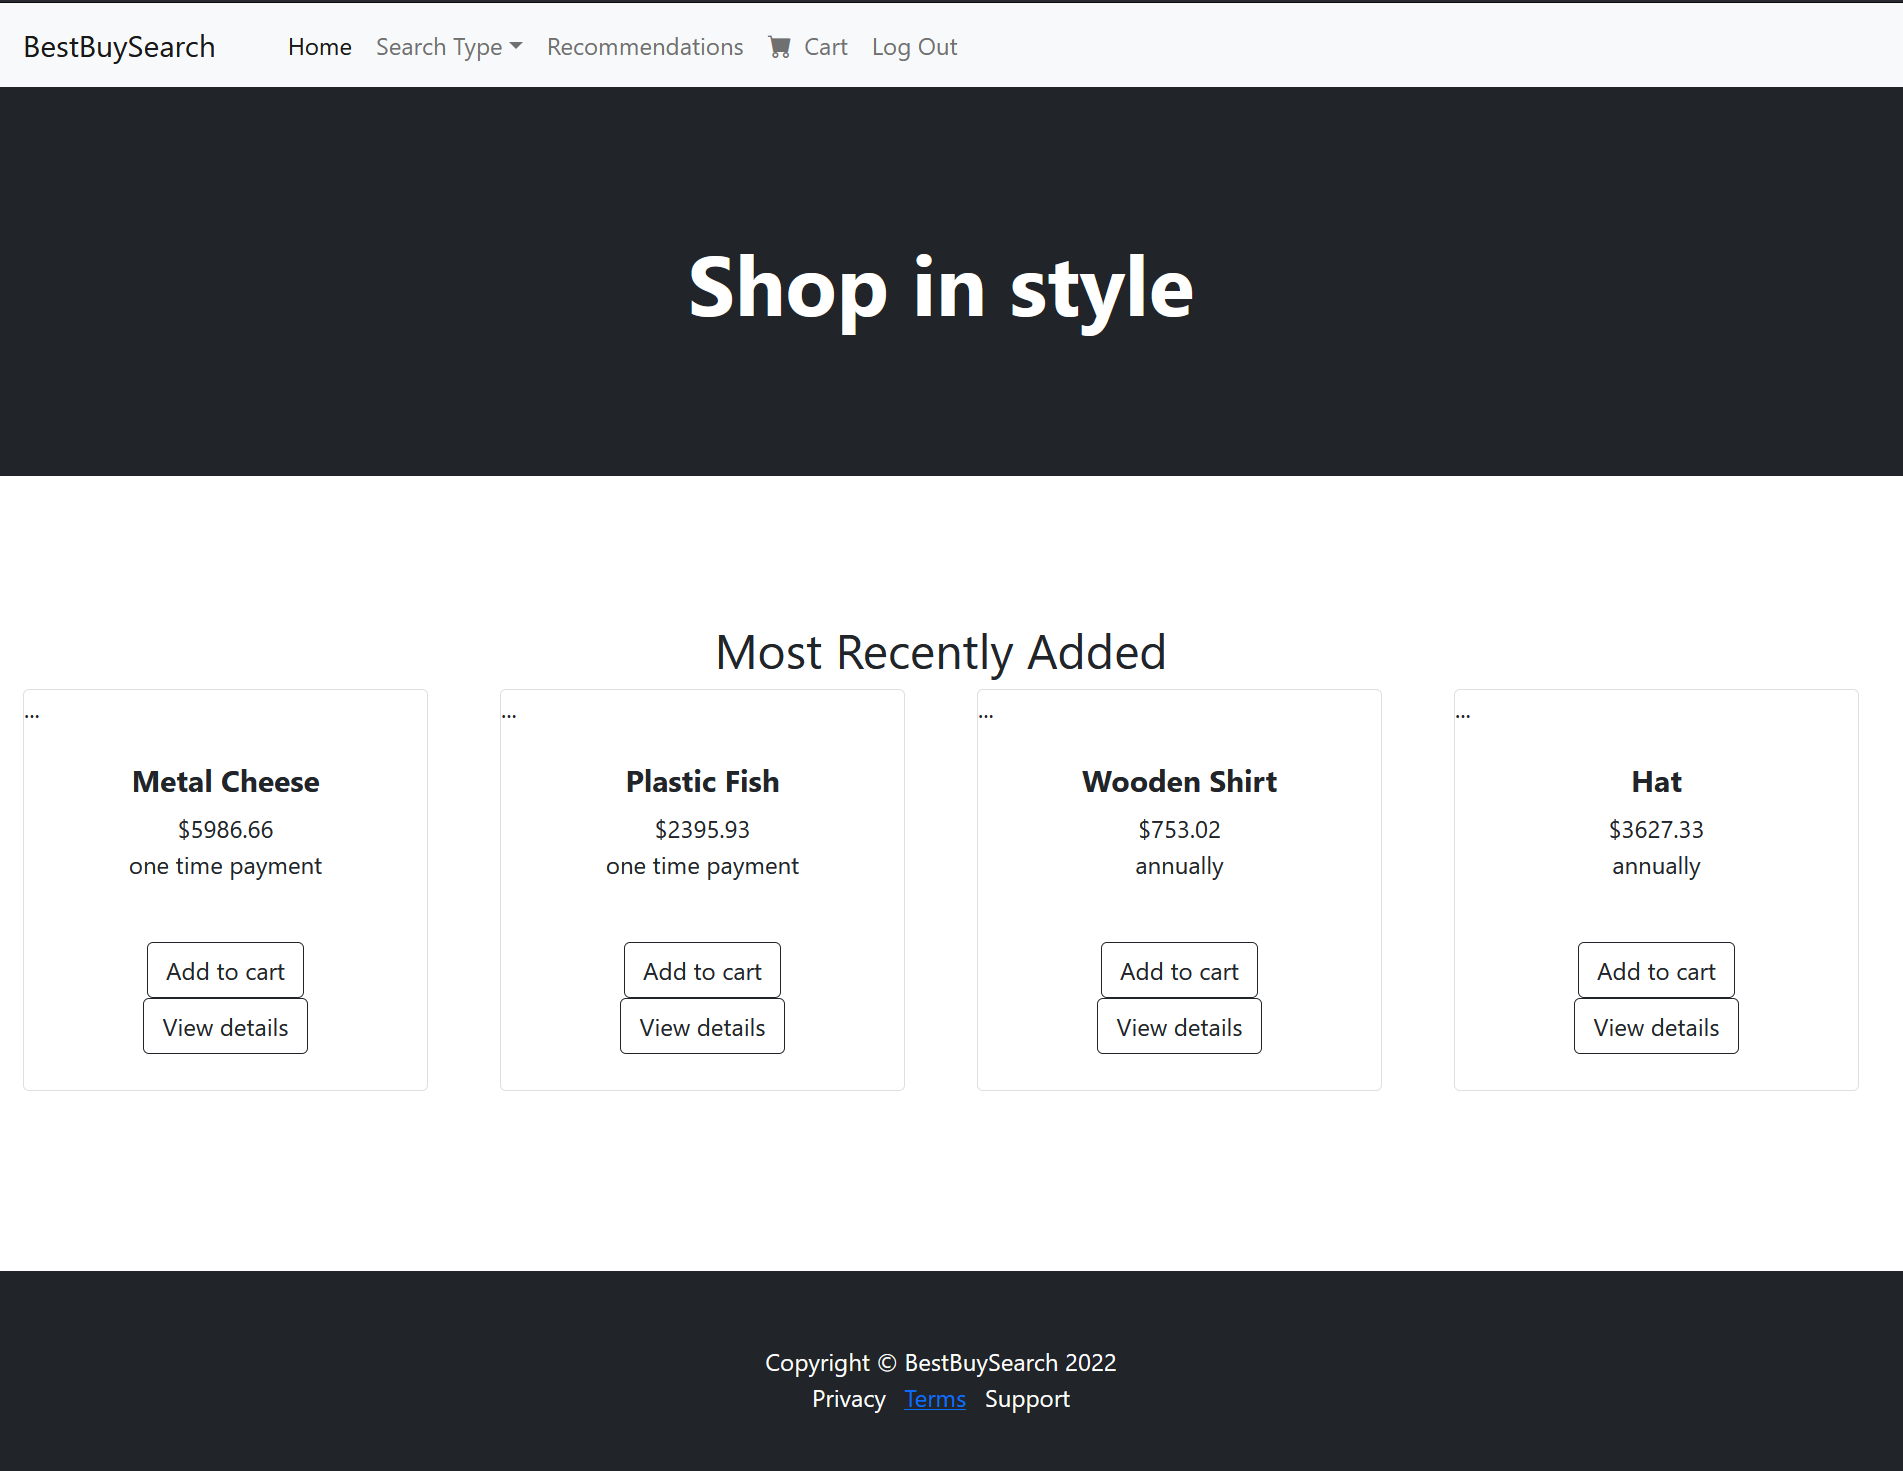
\includegraphics[scale=0.2]{ProductsHomepage.PNG}
    \caption{Store Homepage}
    \label{fig:my_label}
\end{figure}

\paragraph{As seen at the bottom of the page, there's two other unused links surround "terms". Future expansion should consider activating these and bringing up external pages relevant to user privacy rights and a support page for users with issues to contact IT or answer commonly asked questions. }

\subsection{Searches}

\paragraph{All three searches have multiple aspects in common. They are accessible to both user types, have a pagination of 20, display products across the page, and use a button to initiate searching. Searches are performed across the entire VendorProduct table. The Exact and Similar searches use a search bar with user input to find items through their name or category. When navigating to the exact and similar search pages, they display the results of a search by empty string. Meanwhile, the requirement search utilizes drop-down fields with various predetermined choices, and displays all products that fit the default specifications when the page is navigated to.}     

\subsubsection{Exact search}

\paragraph{The exact search uses a case-insensitive SQL query to return the precisely searched for item through name or category.}  

\begin{figure}[H]
    \centering
    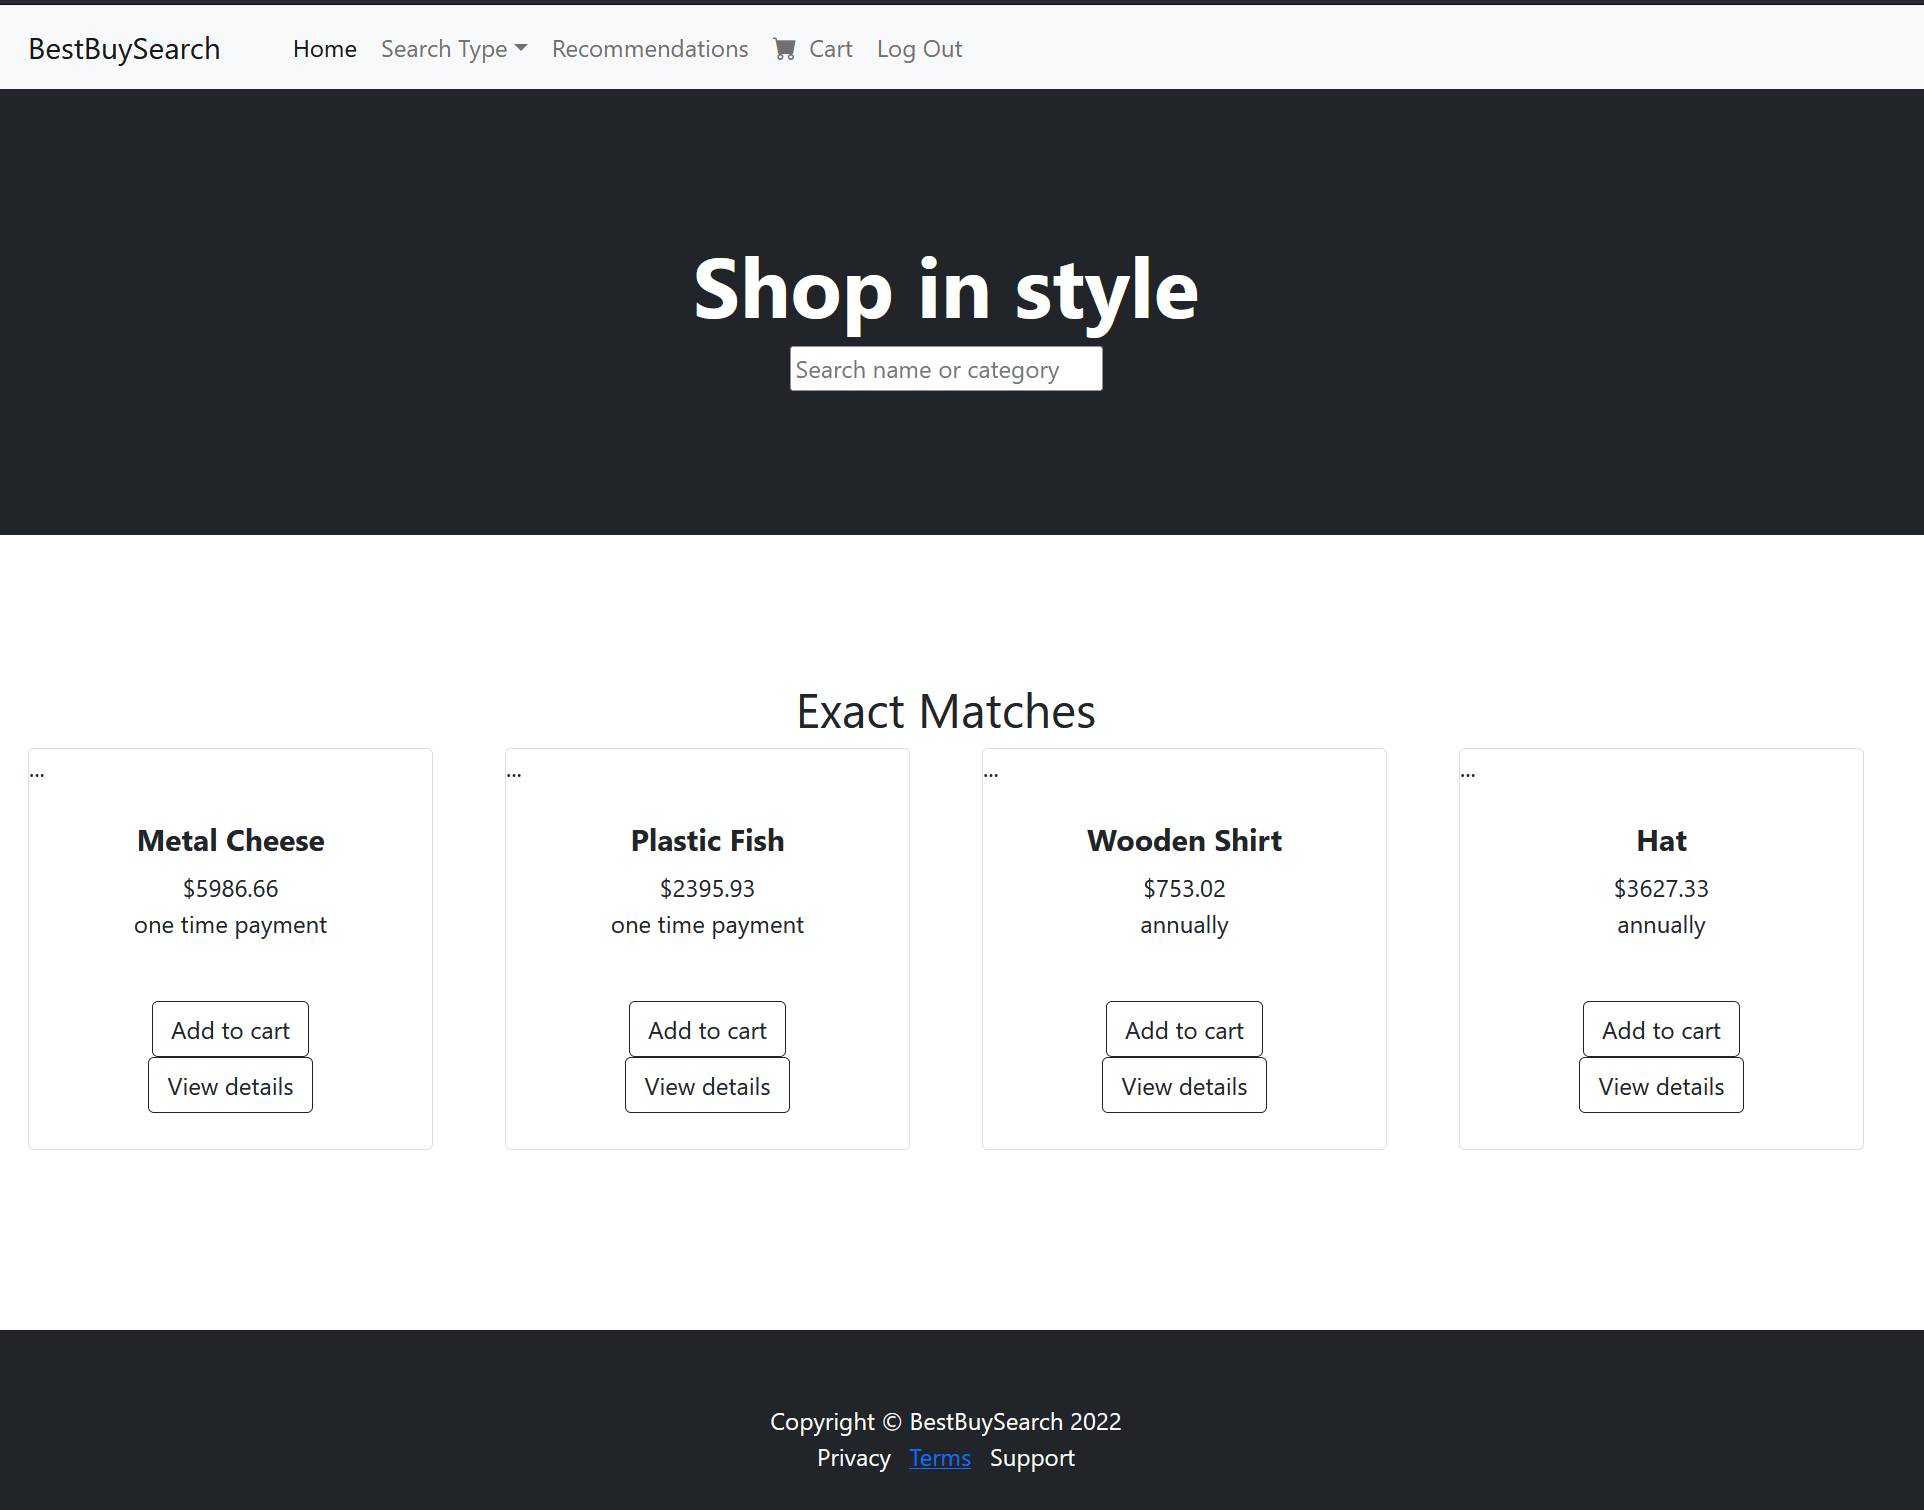
\includegraphics[scale=0.2]{ProductsExact.PNG}
    \caption{Exact Search}
    \label{fig:my_label}
\end{figure}

\paragraph{Searching through exact specification fulfills the customer's desire for a "specific product they want" as outlined in the Course Project description [1]. Development for the exact search was merely following a tutorial on how to implement a search bar in Django. Although, after implementing the requirement search, the category search had to be altered since the category was now an integer field. }

\subsubsection{Similar search}

\paragraph{ Similar search uses a case-insensitive "contains" SQL query to return searched for items through name or category. The SQL query essentially acts as a sub-string search ignoring case. } 

\begin{figure}[H]
    \centering
    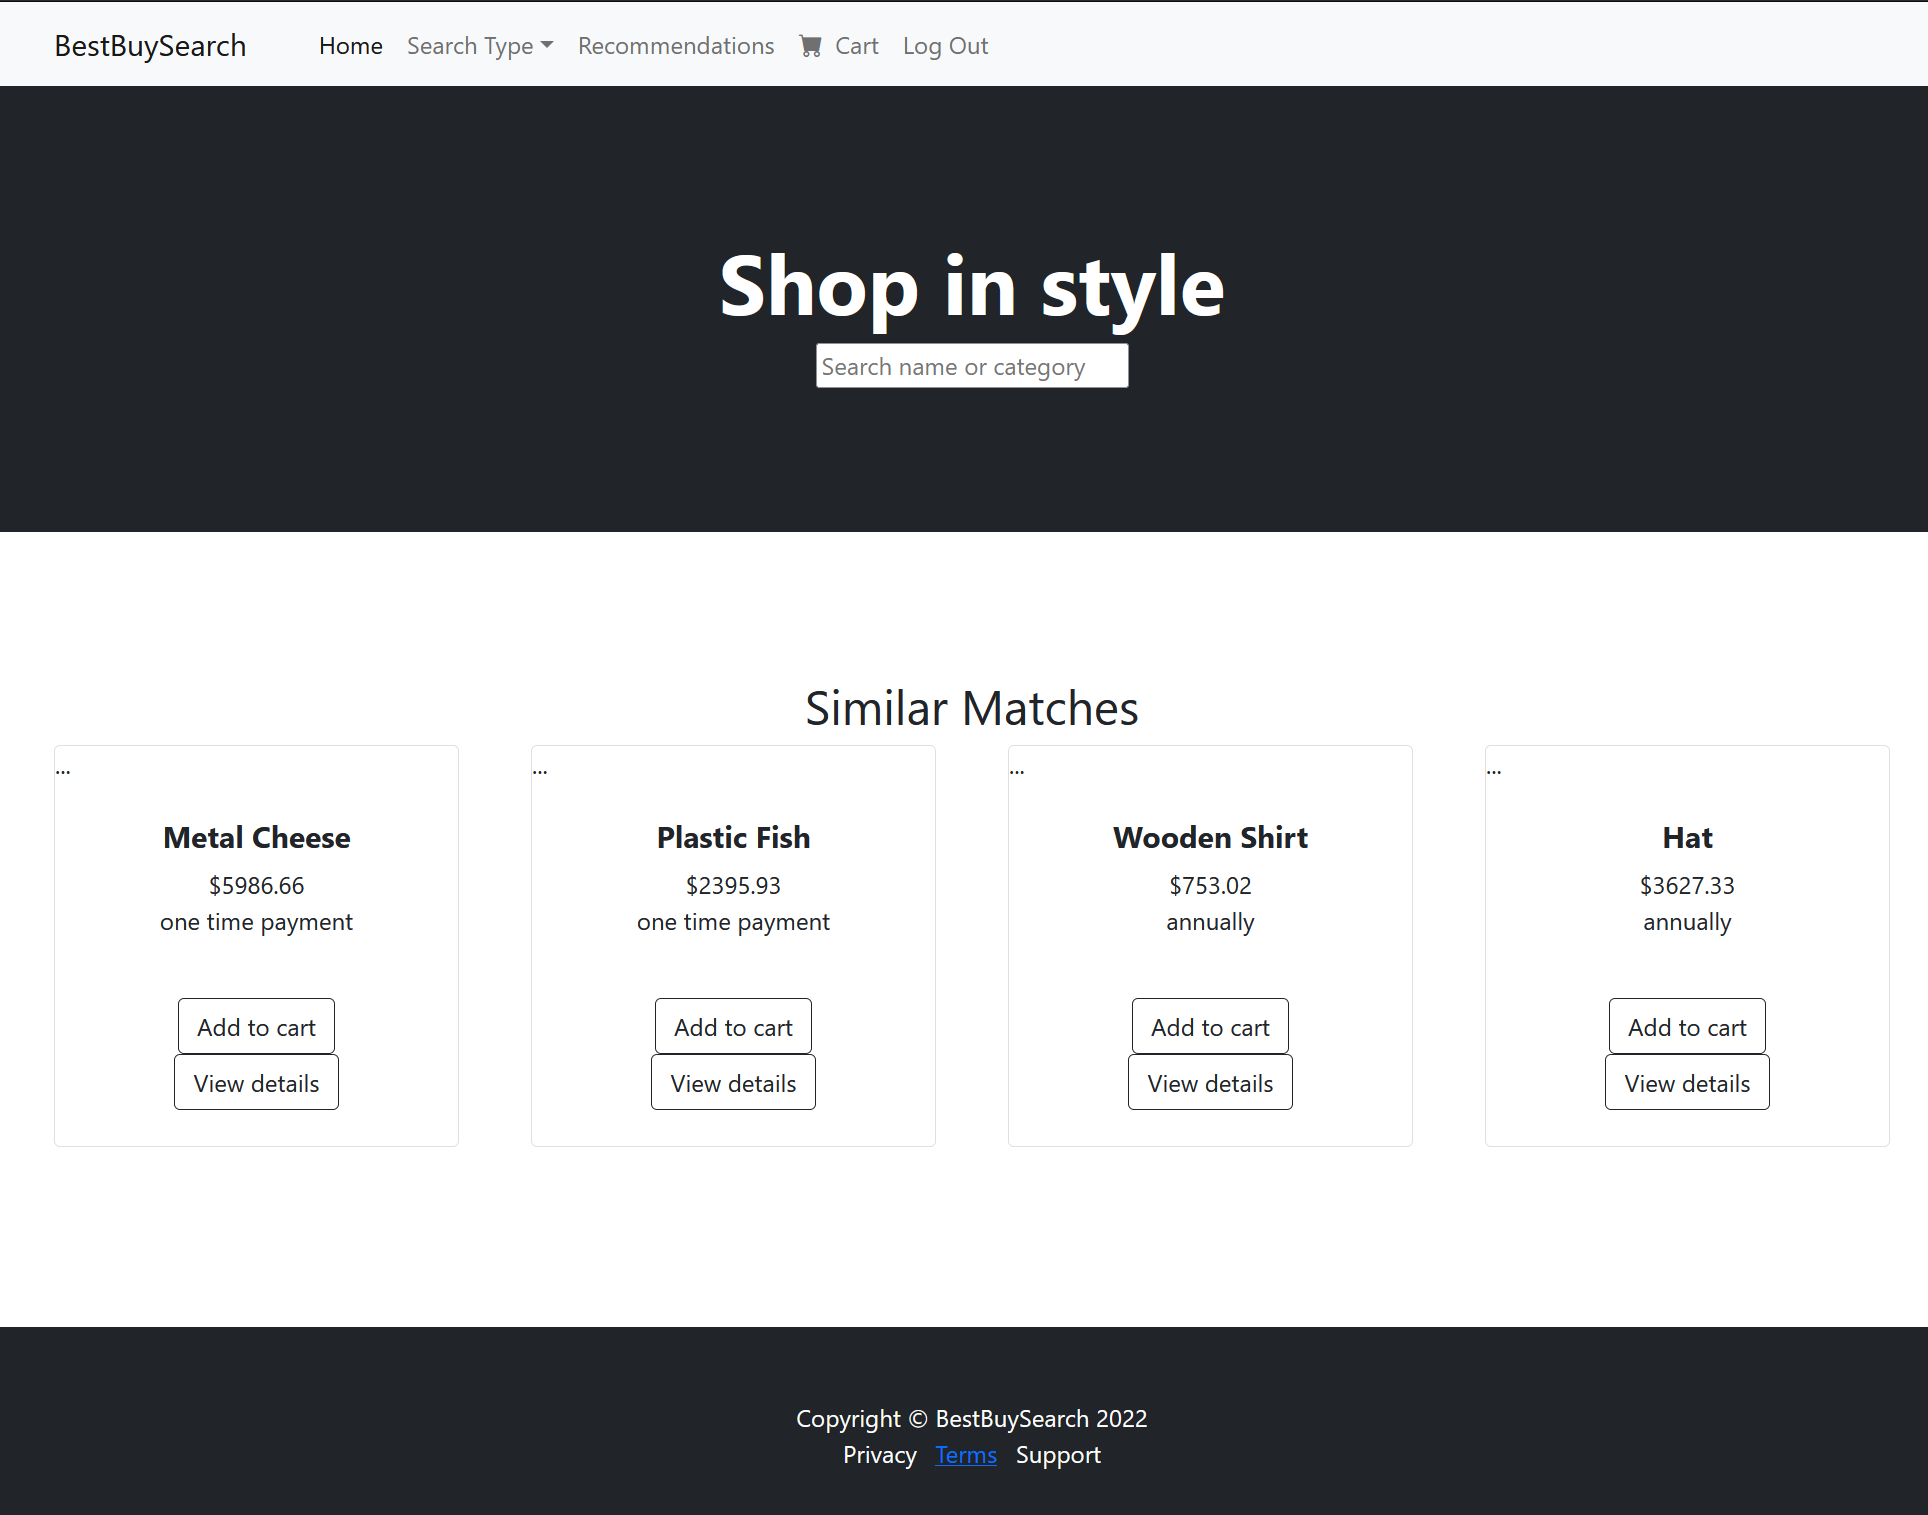
\includegraphics[scale=0.2]{ProductsSimilar.PNG}
    \caption{Similar Search}
    \label{fig:my_label}
\end{figure}

\paragraph{ Although not completely necessary according to the Project Description, the similar search helps the user find a closely matched item. More will be discussed about fulfilling the closest match wish-list below, since that requirement is more closely related to the Requirement search section. } 

\paragraph{ Developing the similar search meant copying and altering the exact search implementation. Similarly to the exact search, the category search was also changed after implementation of the requirement search. Which resulted in only one category being matched at a time. For example, if we had the categories "Editing" and "Edition Management", a similar search given the input "ed" would arbitrarily pick one of the two categories to display items from. Even though both categories have "ed" as a sub string. Ideally, both categories would be displayed, but this was one of the downfalls of implementing choice fields as integers instead of strings. }

\subsubsection{Requirement Search}

\paragraph{ The requirement search combs through multiple columns with a single button-press. It serves as a "closest match of product or service description based on a priority criteria on multiple axes," since that's what's requested in the Course Project description [1]. Additionally, it also allows for different item orderings through user input. }  


\begin{figure}[H]
    \centering
    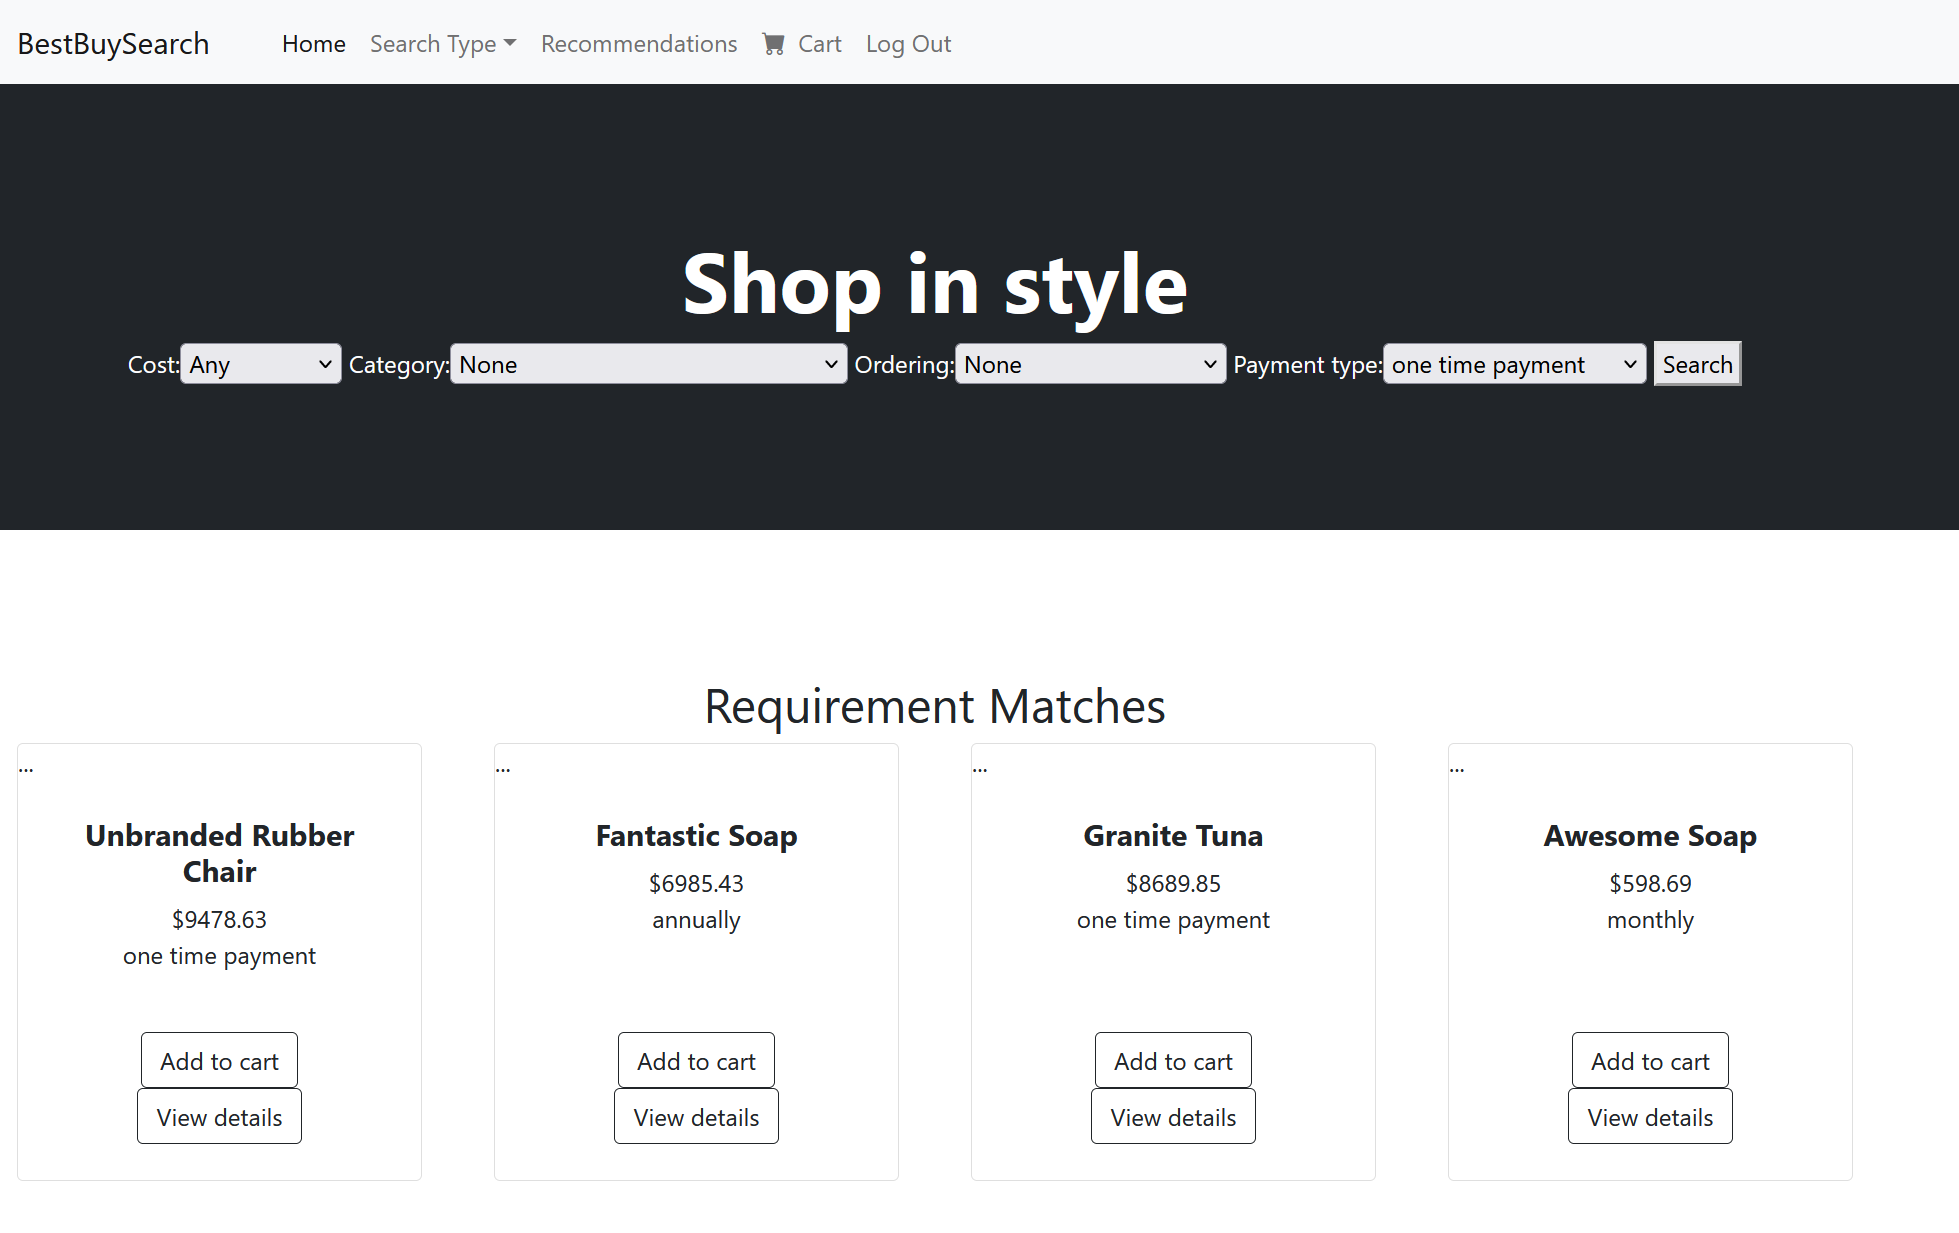
\includegraphics[scale=0.2]{ProductsRequirement.PNG}
    \caption{Requirements Search}
    \label{fig:my_label}
\end{figure}

\paragraph{ Development was much different than the exact and similar searches, since a direct tutorial on how to implement a multiple axis search was difficult to come across. So, experimentation along with scouring the Django documentation was performed. A big portion of the VendorProduct model, such as the category and payment type fields, was changed to accommodate for user choice selection. Implementing the fields as integers mapped to words within Django allowed for easier searching through these fields and creating fake data. Moreover, the addition of predetermined choices made vendor creation of new items simplistic. }      

\subsection{Recommendations page}
\paragraph{ The recommendations page is only accessible to customer users. It works in a relatively simple fashion. It takes all the products within the customer's cart and recommends products that are mentioned, by name, within the brief or full product description of those cart items. It does this through performing a case insensitive sub-string search. Other recommended items are items not within the customer's cart, that mention or contain any cart item's name within their brief or full product description. The retrieved products for recommendation are then ordered by price from low to high to assist customers in saving money. }  

\begin{figure}[H]
    \centering
    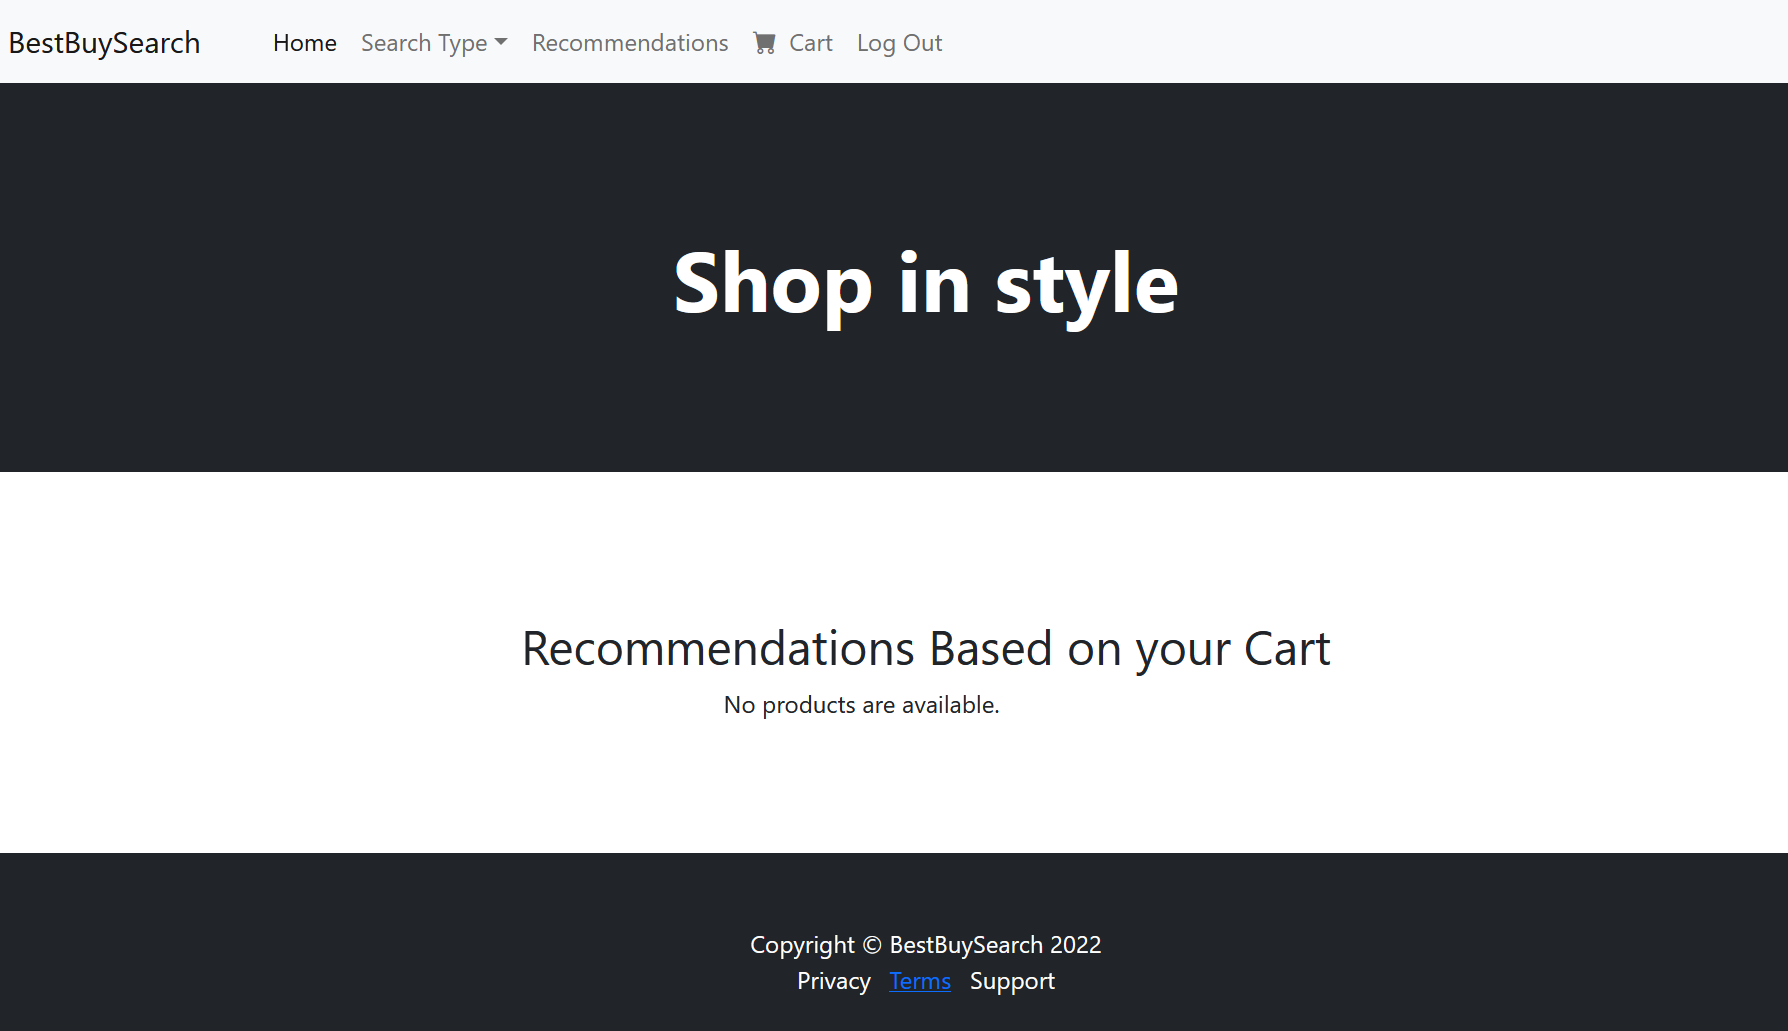
\includegraphics[scale=0.2]{Recommendations.PNG}
    \caption{Recommendations Page}
    \label{fig:my_label}
\end{figure}

\paragraph{ The purpose of the recommendations page was to fill the need for the "requirements wish-list" as outlined in the Course Project requirements [1]. Although, it admittedly loosely fits the specifications. The product matching service independently finds the customer more products, but the recommended products don't necessary match with customer needs. Despite that, Best Buy Search does "protect the customers from overpaying for a service or product" through its ordering of products by price from low to high [1]. It also recommends items related to the ones the customer shows interest in. }

\paragraph{ The above outlined approach may seem primitive, but it's justifiable when considering the other complex aspects of the project. When initially approaching the "requirement wish-list" project requirement, extensive research was performed. The best and proper way to develop a recommendations page was through creating a machine learning model for deploying a recommendation system. Scouring the internet brought up little in regards to pre-made, general purpose systems. So, the crafting of it would have been from scratch. Weighing the pros and cons, it was decided that fleshing out the rest of the project was more important. For future development, implementing such a recommendation system, along with several other model fields to work alongside it, should be considered. }   

\subsection{Customer cart and checkout page}

\paragraph{ The customer cart is displayed underneath the checkout page, so they're both discussed in this section. Another reason for their grouping is the lack of functionality concerning the checkout page. The checkout page currently serves as a method for displaying vendor products that the customer has added to their cart, but it also plays the role of a placeholder for future website expansion. The "checkout" button and the rest of the fields on the checkout page are merely a bootstrap template. No functionality for saving user-entered data or actually "checking out" is implemented. }    
\begin{figure}[H]
    \centering
    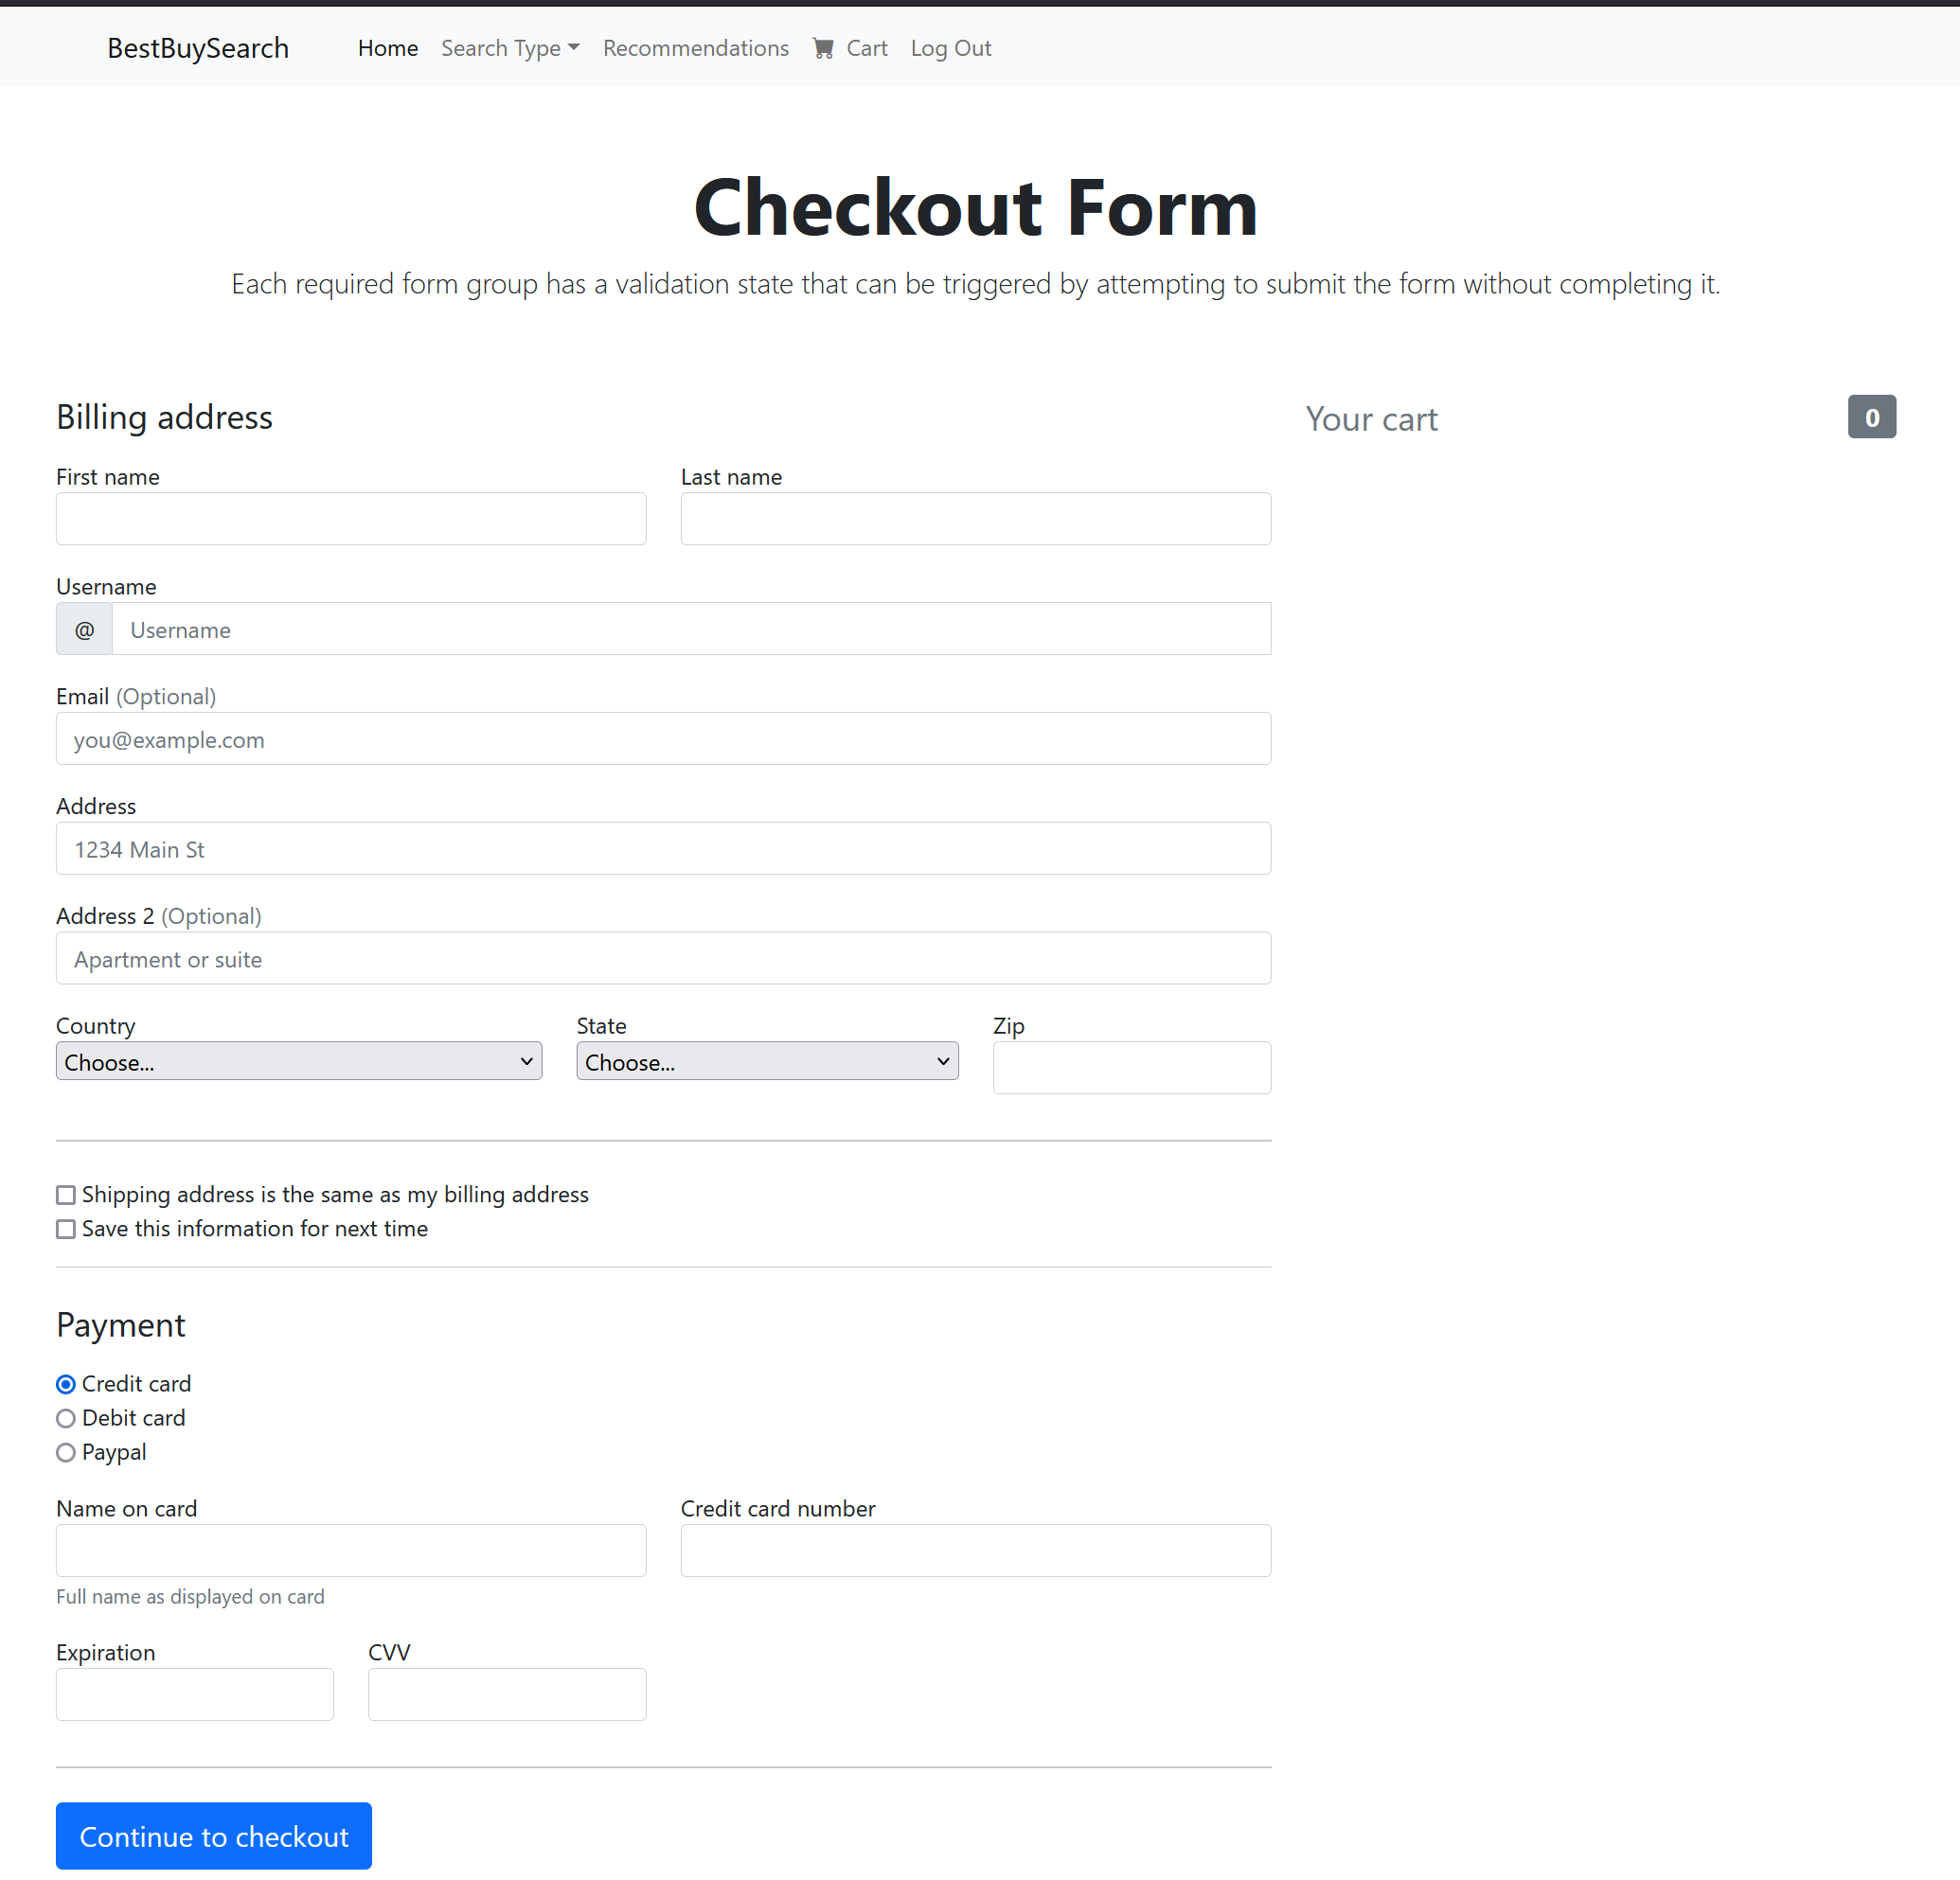
\includegraphics[scale=0.2]{Cart.PNG}
    \caption{Cart and Checkout Page}
    \label{fig:my_label}
\end{figure}

\subsection{Vendor action}

\paragraph{ Vendors can perform a variety of actions and have a "higher" permission level than customer type users. According to the presented specifications, the website for CS360 needed to perform all four of the CRUD operations. The CRUD operations are Create, Read, Update, and Delete. Reading of vendor products is accessible through either user type using one of the mentioned search methods. Deletion is also accessible to both users through customers removing items from their cart, and, as will be seen shortly, vendors can delete products from the database. The incorporation of the CRUD operations of Create and Update are restricted to only vendor level personnel. } 

\subsubsection{Add items}

\paragraph{ Only vendors can add items to Best Buy Search. When they create a new item, they're linked to it through the automatic filling out of the "created\_by" field within the VendorProduct table. Another automated feature of new item creation is the "update\_date" and the "publish\_date", which the vendor cannot manually set and are filled in for them when the new item is created. }   

\begin{figure}[H]
    \centering
    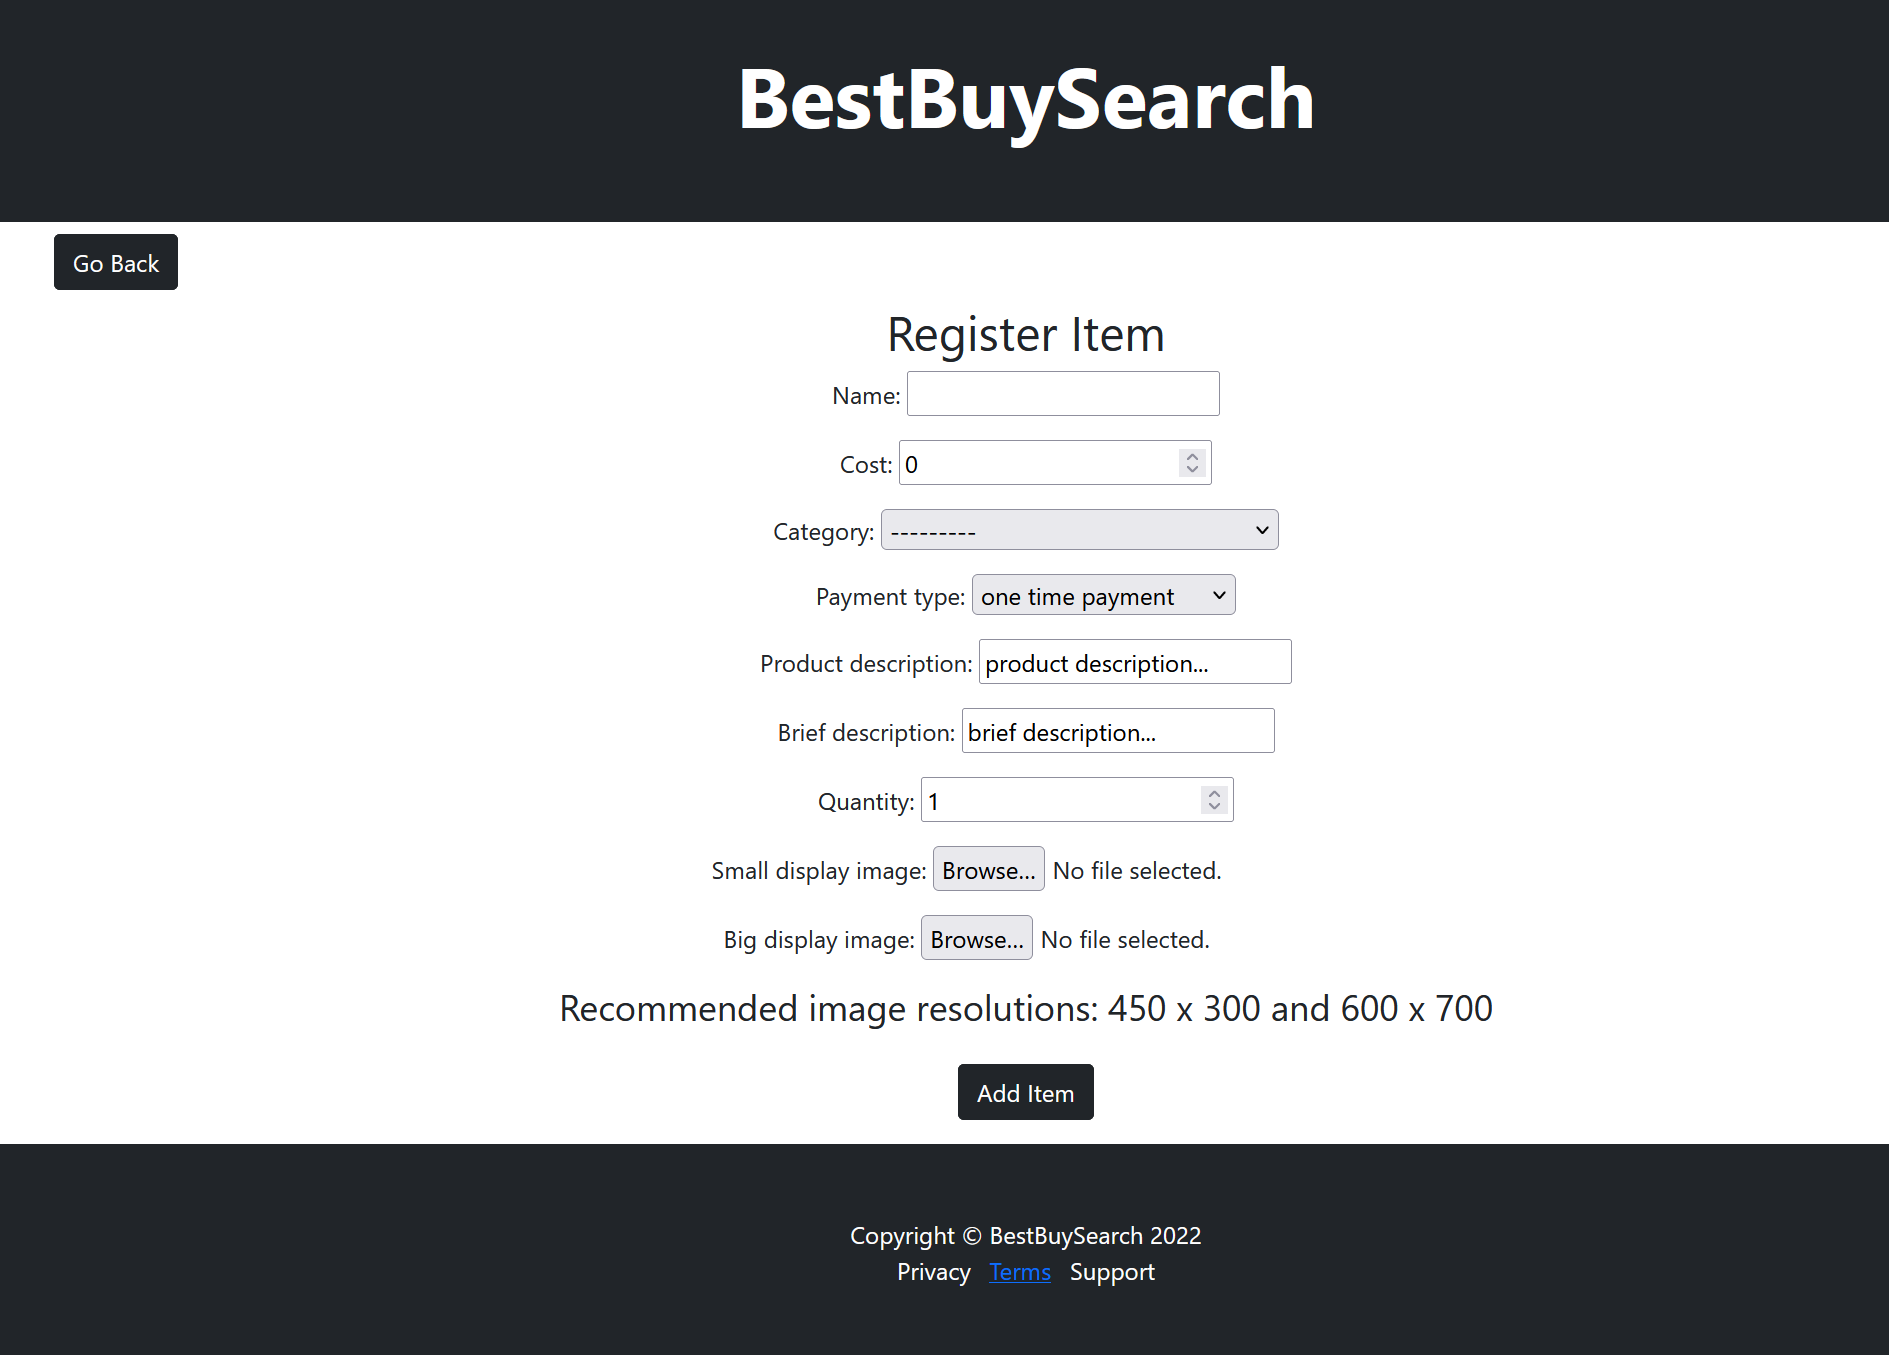
\includegraphics[scale=0.2]{VendorAdd.PNG}
    \caption{Vendor Add Product Page}
    \label{fig:my_label}
\end{figure}

\subsubsection{Edit/Delete items}

\paragraph{In addition to adding new items to the product table, vendors can also edit the items that they have listed on the site, which accounts for the update operation of CRUD. From the shop menu drop-down, a vendor can select a vendor action option to edit/delete an item. Selecting this option will then bring the vendor to a page listing all of their current published items present on the site. For each of the listed items, the vendor will then be able to choose to edit or delete the item individually. All of this vendor's created items are displayed with a pagination of 40, with the ordering of them as arbitrary. Such a large pagination is used in comparison to the search pages since the vendor item can't be searched through unless done manually. }

\paragraph{Future expansion of this page should implement a mechanism such as a search bar or drop-down options to sift through the items created by this vendor. With the given time constraints, this objective wasn't high on the priority list since it isn't expected for each vendor to publish a large quantity of items. Therefore, the search capability on this page isn't of utmost importance.}

\begin{figure}[H]
    \centering
    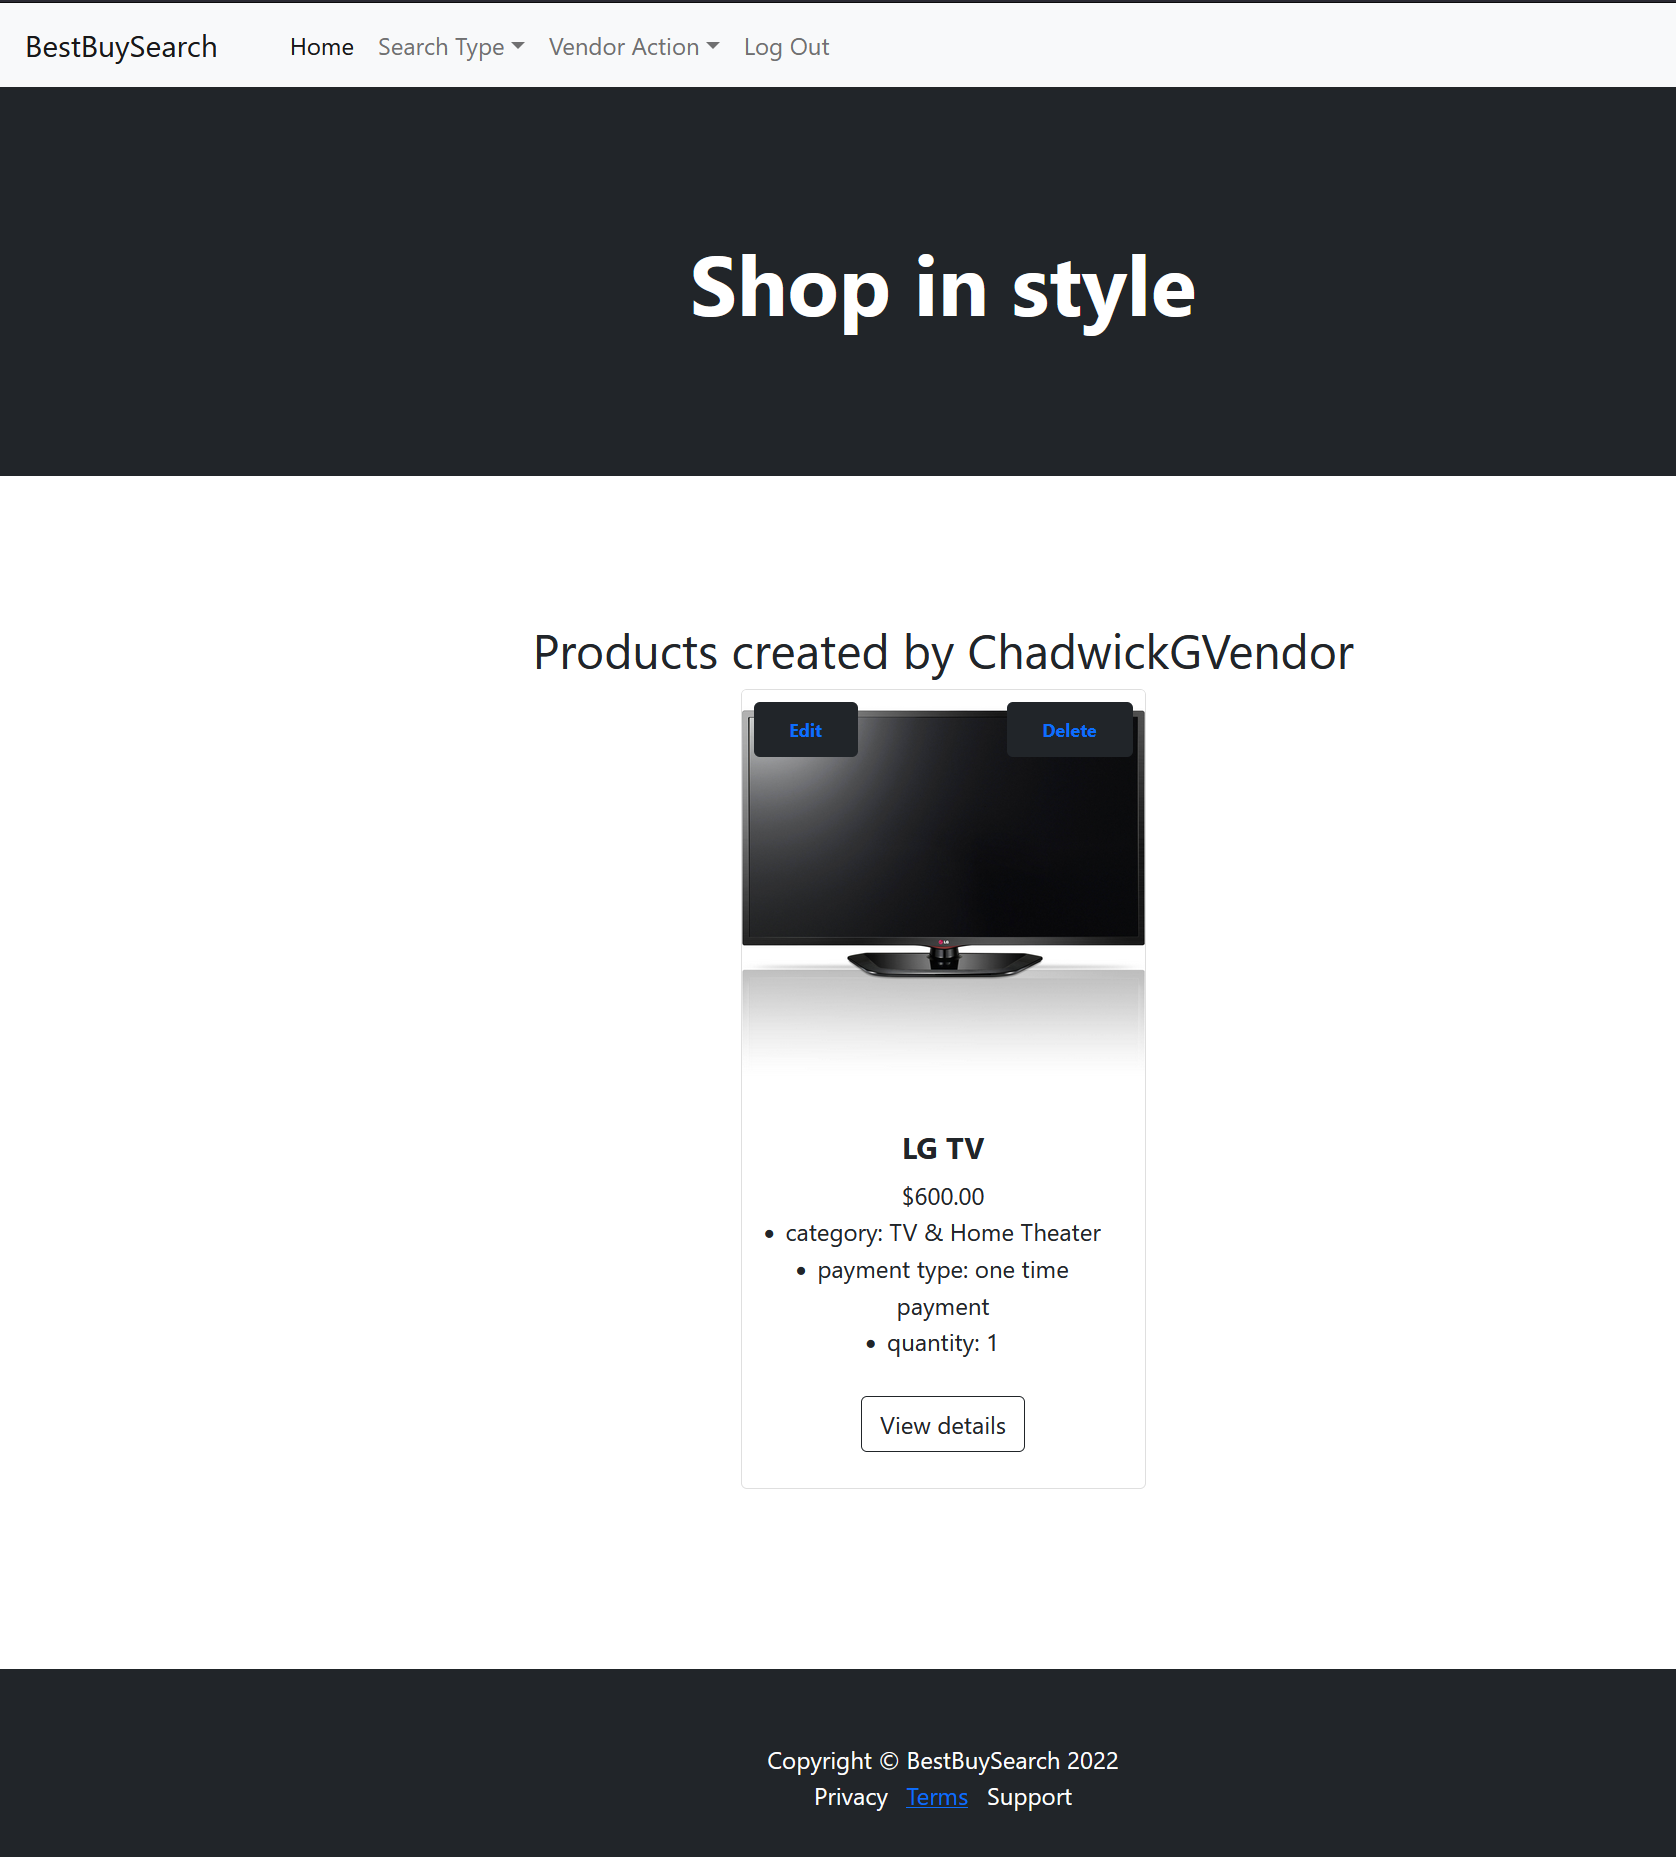
\includegraphics[scale=0.2]{VendorEditDelete.PNG}
    \caption{Vendor Edit/Delete Interface}
    \label{fig:my_label}
\end{figure}

\subsubsection{Edit items}

\paragraph{If editing the item is selected, the vendor is brought to the item's corresponding edit page, show below. Only the vendor who created the item has access to this or the deletion page for their particular items.}

\begin{figure}[H]
    \centering
    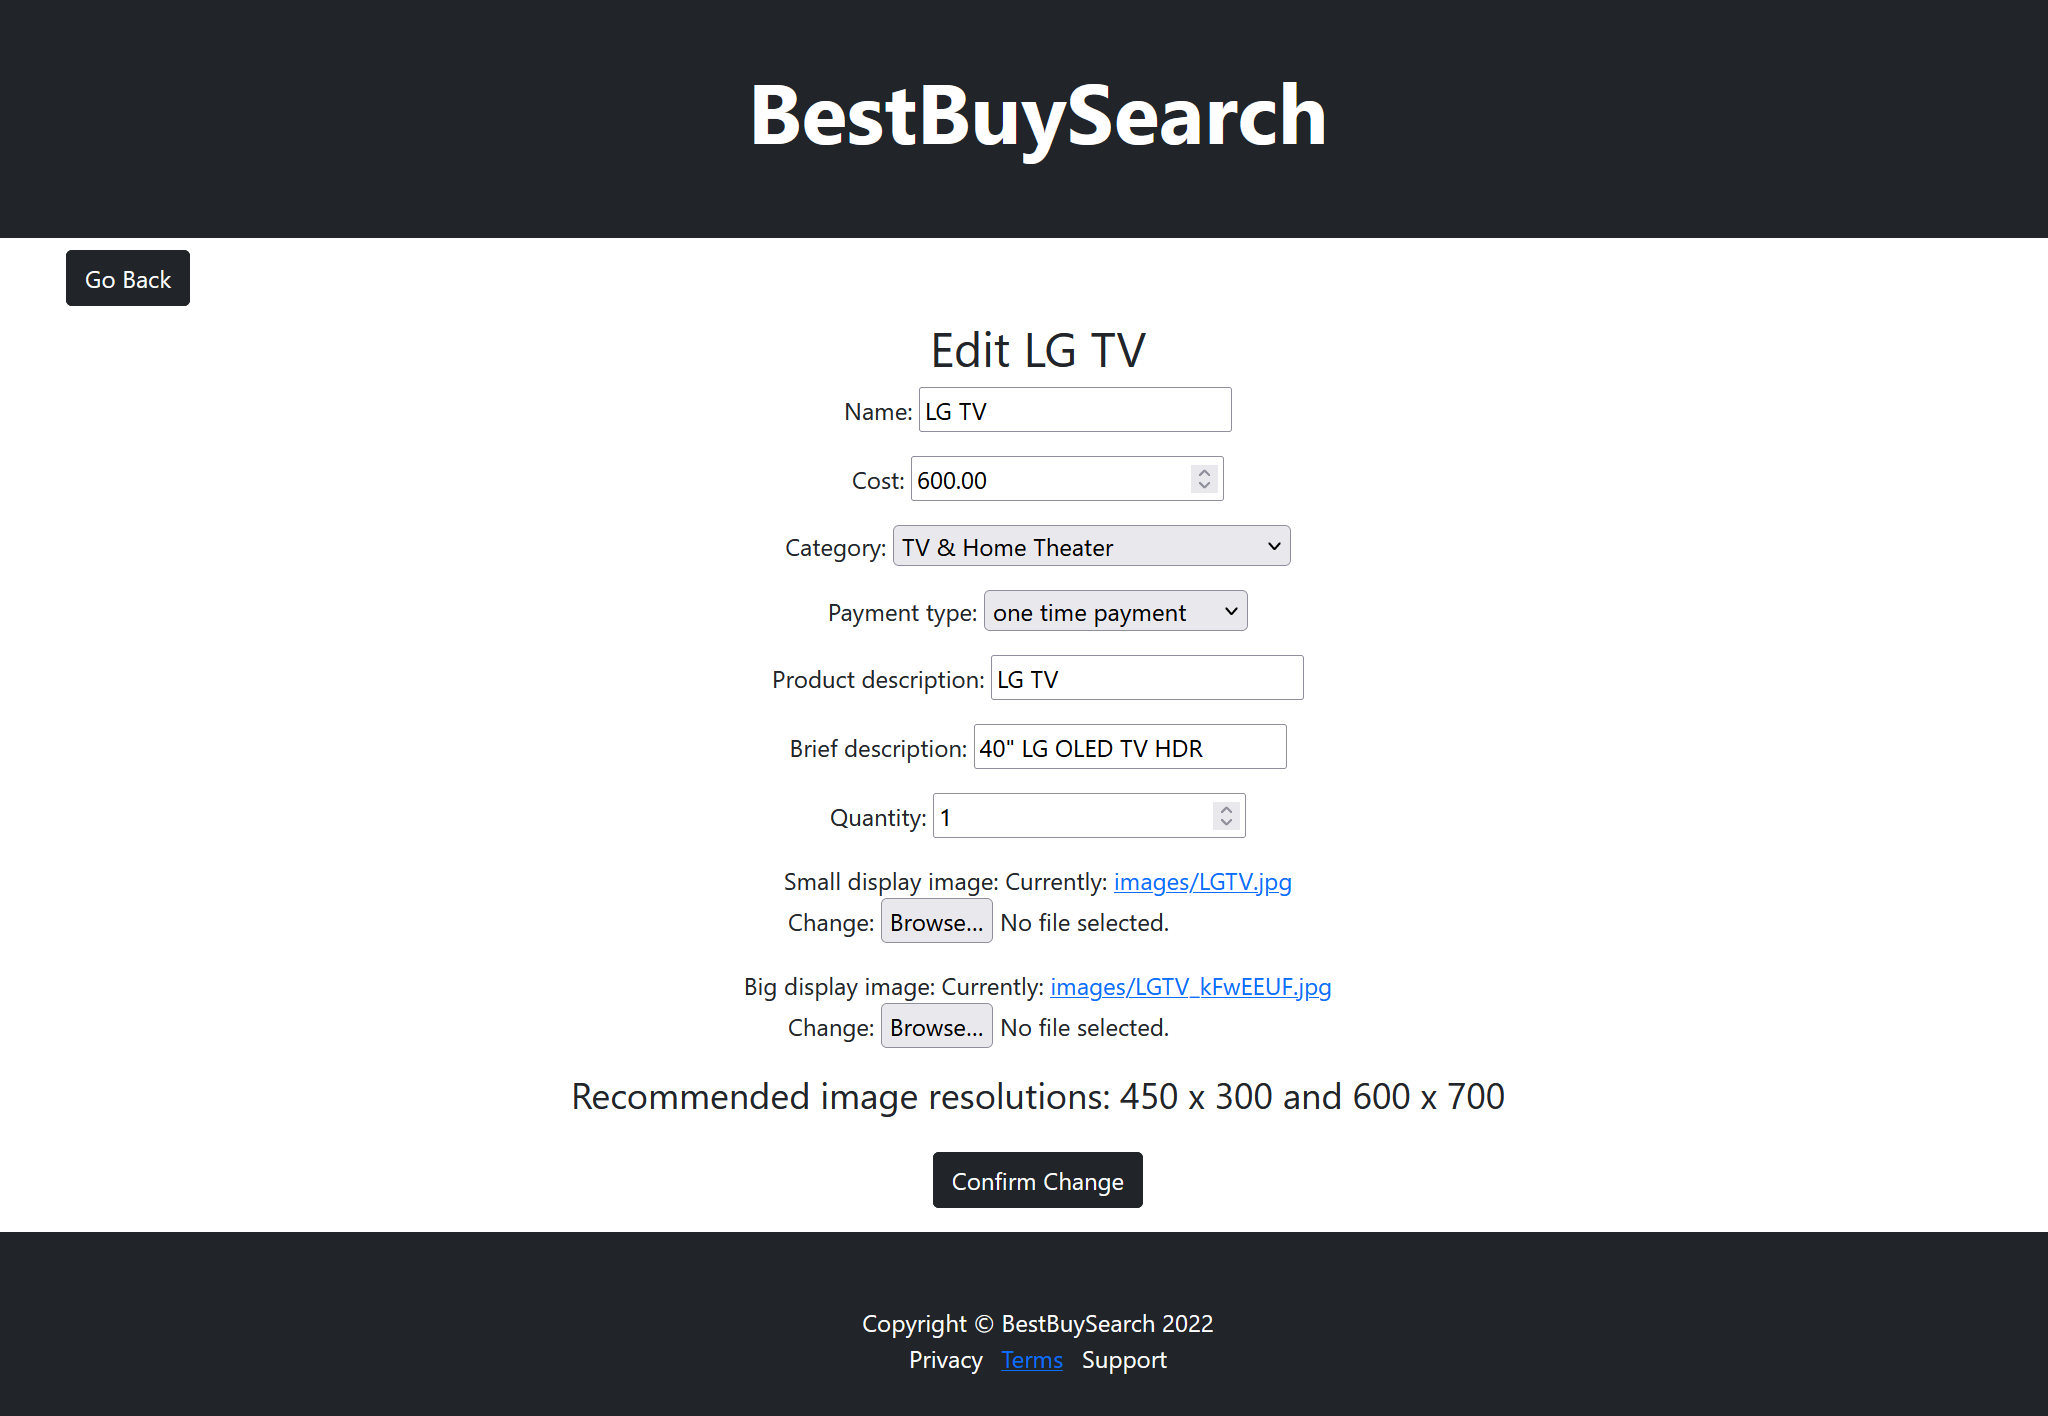
\includegraphics[scale=0.2]{VendorEdit.PNG}
    \caption{Vendor Edit Page}
    \label{fig:my_label}
\end{figure}

\subsubsection{Delete items}

\paragraph{Furthermore, deletion being one of the simpler operations to implement, the implementation of this within the user interface is rather straightforward. The website requests a confirmation from the vendor that they would like to remove the product from the database and the store homepage before executing the deletion.}

\begin{figure}[H]
    \centering
    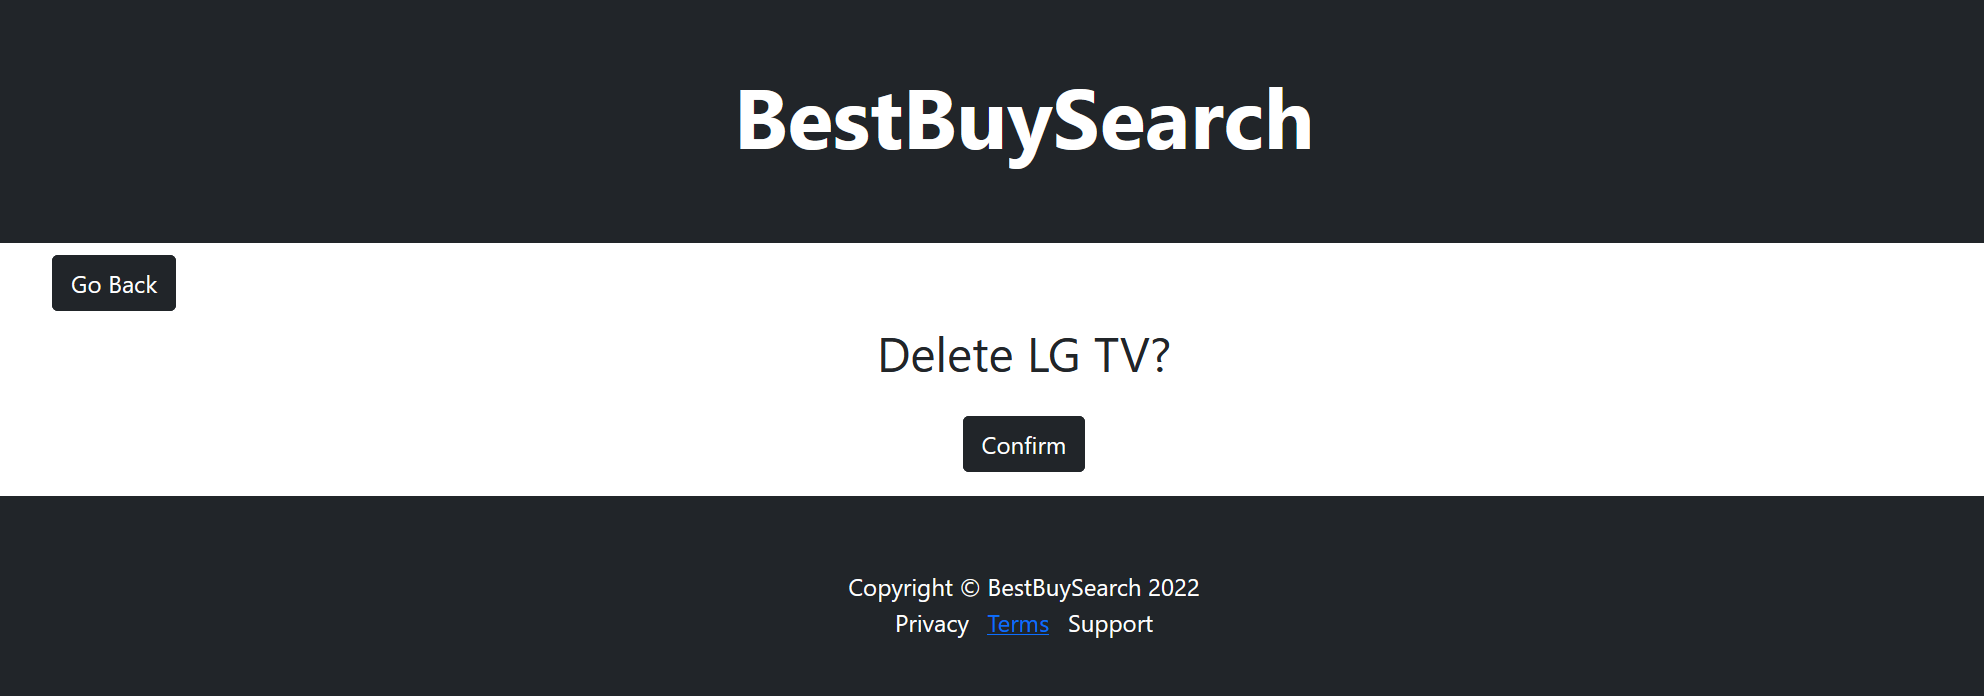
\includegraphics[scale=0.2]{VendorDelete.PNG}
    \caption{Vendor Deletion Confirmation Page}
    \label{fig:my_label}
\end{figure}


\section{Database population with Faker}

\paragraph{ Faker was used to populate the database with randomized fake data through running a custom command. The custom command can be run through typing "python manage.py createdata" with a given integer argument. The given number of products are created in the database linked to a newly created fake vendor. }  

\subsection{Data generation script}

\paragraph{ Manufacturing the data generation script "createdata.py" involved the creation of a custom Command class extending from the pre-established BaseCommand class. Implementation of the "add\_argument" method was used to allow registration of additional arguments passed in through the command-line. In addition, the "handle" method was necessary to enact the command's functionality of creating a randomized new vendor user and the desired number of vendor products. As seen in the provided images, most items have reasonable and descriptive names. Such naming couldn't be achieved using default Faker Providers, so a third part provider called "faker-ecommerce" was installed. }     

\paragraph{ One of the downfalls of using Faker for the data generation script concerns how a method for generating fake images wasn't found. Since each vendor product requires both a small and large display image, the image field for the fake products are filled with manufactured image urls that don't link to actual images. Therefore, displaying the fake test data on the website is rather lackluster since image fields are left blank. This shortcoming is made obvious when looking at the images below. This problem affects both the normal product display and the product detail pages. }

\begin{figure}[H]
    \centering
    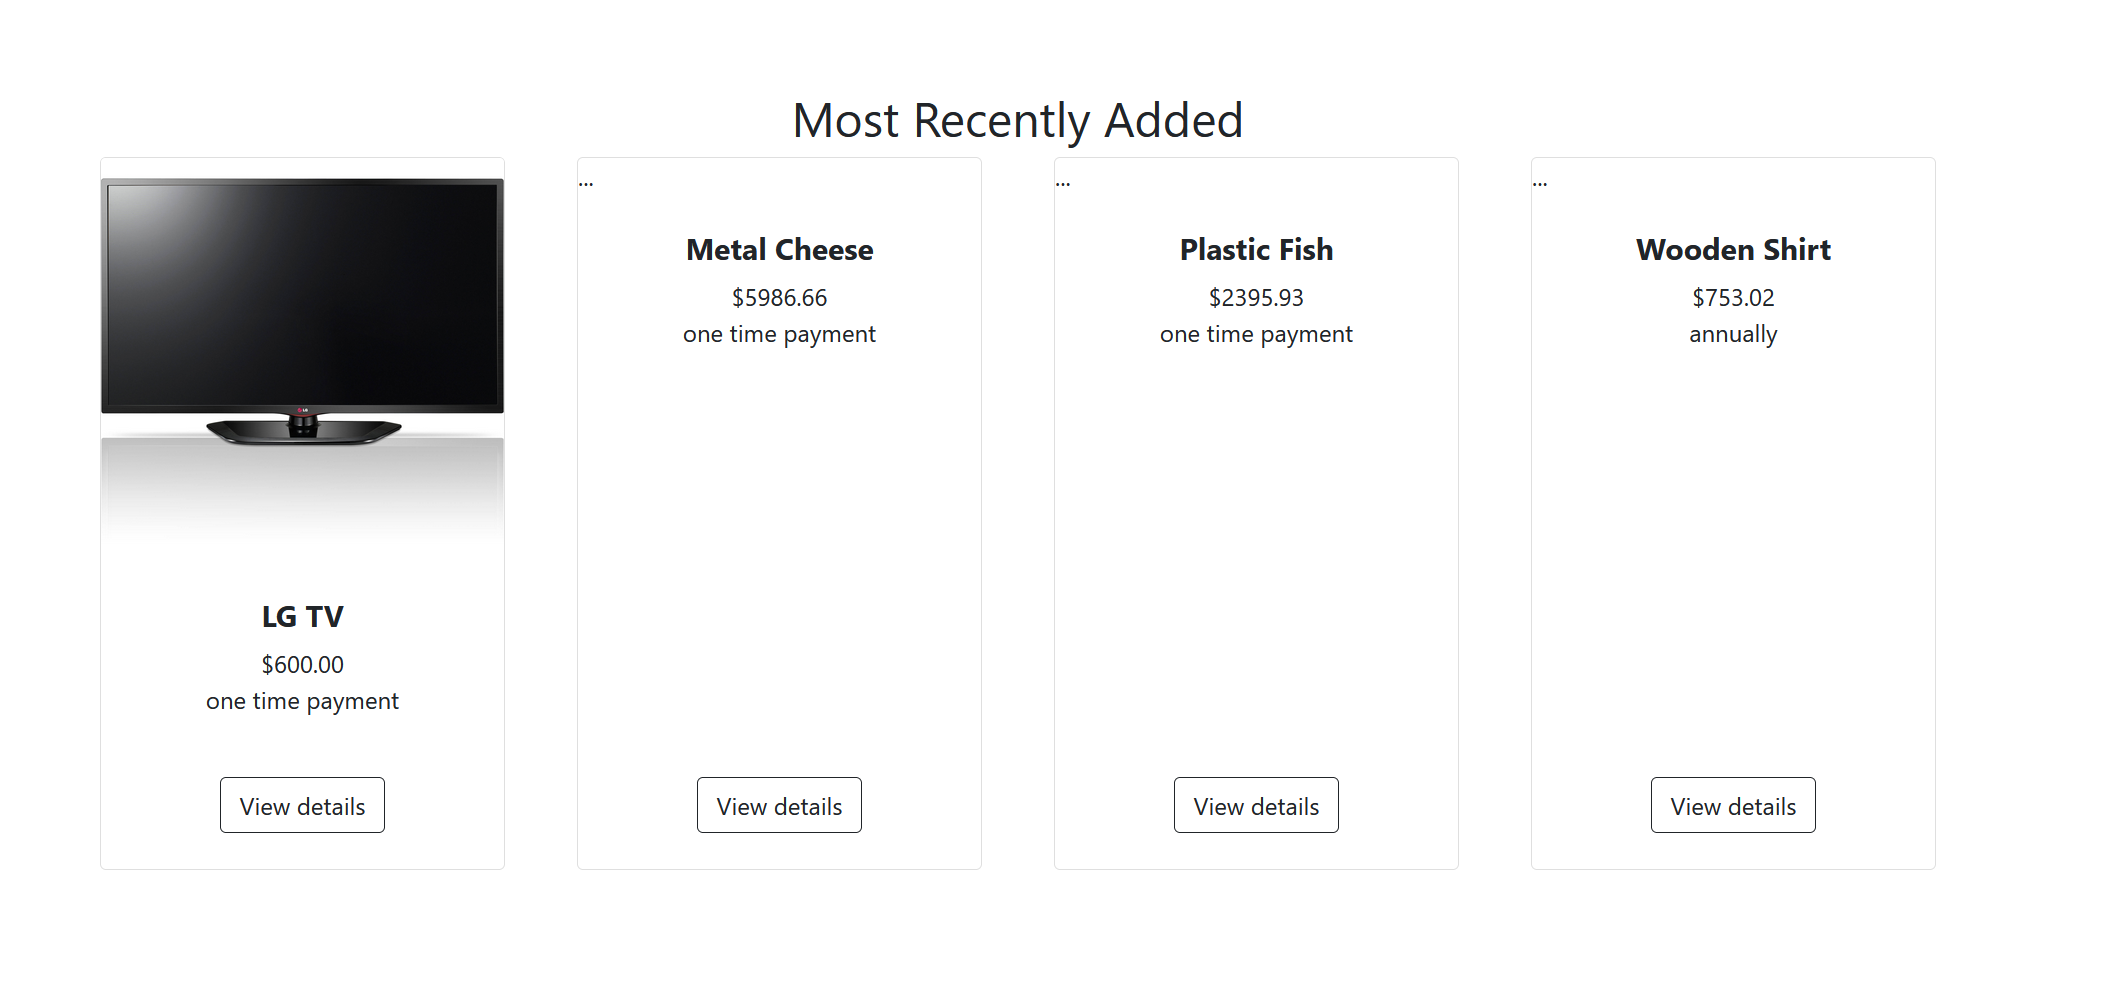
\includegraphics[scale=0.2]{VendorCreatedVFaker.PNG}
    \caption{Vendor Created Product Vs. Faker Generated Product Comparison}
    \label{fig:my_label}
\end{figure}

\section{Pagination}

\paragraph{ After populating the database with fake data, handling big amounts of vendor items became a more relevant issue. In response to this, each view displaying items, besides the home page, needed to be paginated by a certain amount. Otherwise, huge amounts of display data would slow down the load time of the Best Buy Search website's pages. Carrying out pagination was simple since it's a common solution in web development. Although, the method used didn't seem to work when unordered data was presented. Therefore, all data not already ordered was organized by product id in descending order. }

\section{MySQL Queries}

\paragraph{ The only database queries dealt with were those generated by Django migrations. These migrations were created through making changes to, or adding new, database models. Which would then be translated into a MySQL query applied to the local database in PHMyAdmin when migrating changes. These migrations helped both team members stay on the same page, since even without putting the project onto a website, both people's databases were structured the same. } 

\section{Decorators}

\paragraph{ Throughout the Best Buy Search site, user permissions play a crucial role in how the site is structured and can be navigated. Therefore, implementing security to ensure that web pages can't be accessed by those without the correct permissions is crucial to database integrity. For example, if a user without a vendor or customer id tried deleting an item from the database, the database should fail to delete the item but Django may not recognise that and stop displaying it anyways. Two decorators were designed with this specific purpose in-mind, and each serve to redirect unauthorized users to the login page if the user tries to manually enter a protected web page's url. They're implemented as apart of each web page's view. One decorator is needed for each user type, but a third built-in decorator that checks if users are logged-in also helps protect web pages accessible to both vendor and customer users. }

\paragraph{ Early on in project development, a third "guest" user type was theorized. In concept, they wouldn't need a login or model, but because of that, the decorator for such a user was difficult to construct. It was dismissed because of the before mentioned and various other complications, and since it isn't explicitly requested by the project description. }

\section{Project Difficulties}

\paragraph{ Most imposing of all, the one project difficulty that affected initial project growth most was figuring out how to approach the project. Laying out a comprehensive plan at the start was nearly impossible, since neither group member had any prior experience with Django or web development. Eventually, this problem was overcome through consulting with the class TA, Kallol, and through independent research. Because of the lack of experience, several features created at the start needed reworking for compatibility with multiple user types.}  

\paragraph{ Another big issue concerned group member involvement. With a lack of structure and infrequent deadlines for the project, it was easy to put off and focus on more pressing matters. As a result, work was heavily  disproportionate between group members. }

\paragraph{ The rest of the project difficulties were mainly discussed in their respective sections above. As an overview, some of the difficulties mentioned were implementing the requirements search to query across multiple field, the similar search in relation to the category sub-string search, reasonable data with Faker, and an accurate recommendations page.  }

\section{Conclusion and Suggestions}

\paragraph{ In conclusion, Best Buy Search is a product and service matching site with a variety of search features, a recommendations page, and checkout page. Logging in is required for site access, and visitors can create accounts as either a vendor or customer user under a binding agreement. Vendors can create, edit, and delete items, while customers can add/remove items to/from their carts. As discussed above, Best Buy Search meets all requirements outlined in the project description for CS360, Database Systems. }

\paragraph{ Most suggestions for improvements concerning the Best Buy Search site were made above. An overview is given to consolidate all of the suggestions in one place. Major suggestions for project improvement include: switching out the username for an email field, removing the is\_vendor and is\_customer fields in the User model, including credit card and address fields in the Customer model, using the brand name for item display and filtering, support and privacy links, allowing multiple category searches in the similar search, adding search capabilities to the display page for the logged in vendor's items, developing a more accurate recommendations page, granting the checkout page functionality, manifesting images to correspond to the faker-generated image urls, and incorporating a third guest user type.  }

\paragraph{ The final recommendation for further development involves storing and altering item quantity. Currently, when customers add an item to their cart, only a single item is ever added. Ideally, there would be an integer input field for customers to decide how many of a product they'd like to add to their cart. Then, that amount would be displayed on the checkout page and be multiplied by the cost of a single item to show how much x number of items will cost the customer. Once checked out, the specified number of items the customer checked out with would be removed from the quantity left of the item in the database. If this quantity ever reached zero, the item would stop being displayed on the website. This idea for future improvement is why vendors can currently publish items with a quantity of zero. }

\paragraph{ A suggestion for future classes would be to have more deadlines for project development. Some points could be moved from the final demo or the first big intermediate demo and contributed toward a couple more "check-in" like presentations earlier on in the course. During the additional demos or check-ins, each group member should be required to point out their contribution since the previous presentation. This is a similar strategy to how the semester long project is conducted in Software Engineering CS 383. Additionally, further instruction or reference material, as could be provided in a lab, for the development of the project would be greatly beneficial.}

\section{ Source Code}
\paragraph{ The source code for this project is available at \\ https://github.com/SethCram/NoMigrations. }

\section{REFERENCES}
 [1] Hasan Jamil. CS 360:  Database Systems. Retrieved May 4, 2022 from https://canvas.uidaho.edu/courses/6701 
 [2] Anon. Documentation. Retrieved May 4, 2022 from https://docs.djangoproject.com/en/4.0/ 
 [3] Anon. Documentation. Retrieved May 4, 2022 from https://www.python.org/doc/ 
 [4] Anon. XAMPP FAQ/Documentation. Retrieved May 4, 2022 from https://www.apachefriends.org/index.html 

%\bibliographystyle{ACM-Reference-Format}
%\bibliography{sample-base}


\end{document}
